\section{Test Results}
We test proposed techinque using the use cased explained in the previouse section.

\subsection{Verification of Results}

From Figure~\ref{fig:TestResults:distance0} we see that the simulation compared to the real-world results from Figure \ref{} is a close match. 
We see the same stop and go behavior as a results from traffic lights, and the arrival times are also a close match. 
If we compare the driving speed of the simulation show in Figure \ref{fig:TestResults:speed0} with the real-world data from Figure \ref{} we see that in most cases the vehicles are either driving at the maximum speed, or they are at a full stop. 
This behavior on the two graphs are almost identical and consistent with the stop and go behavior caused by traffic lights. 
Figure \ref{} shows the distance to a traffic light where each vehicles makes a stop. 
All the blue dots are vehicles that only have a single stop, red squares have two stops and yellow triangles have 3 stops.
The traffic light for this figure is the first junctions driving from Vesterbro. See Figure \ref{fig:Introduction:hobro}. The Figure \ref{} show the real-world data from the same traffic light. 
%TODO: when we have something to compare with

\begin{figure}[htb]
\includegraphics[width=0.5\textwidth]{images/tp0/speed0.png}
\caption{Speed graph}
\label{fig:TestResults:speed0}
\end{figure}

\begin{figure}[htb]
\includegraphics[width=0.5\textwidth]{images/tp0/distance0.png}
\caption{Distance graph}
\label{fig:TestResults:distance0}
\end{figure}

%
\begin{figure}
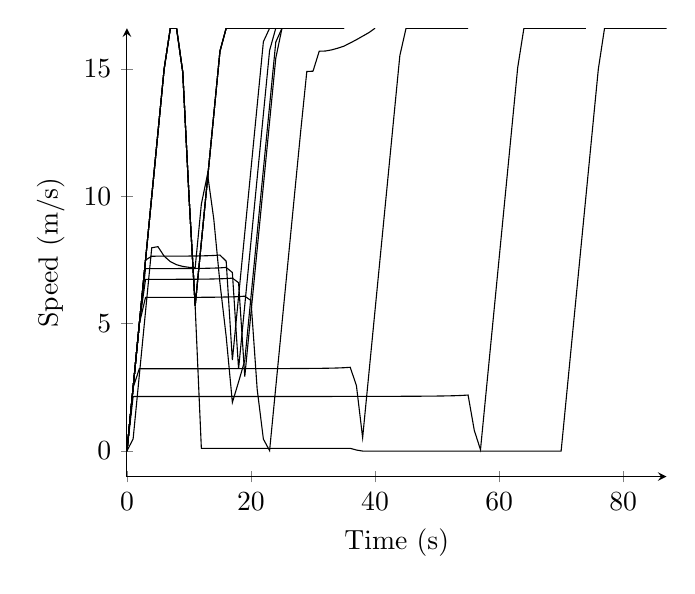
\begin{tikzpicture}
\begin{axis}[
legend style={anchor=west},
axis x line=bottom,
axis y line=left,
ymin=-1,
xlabel=Time (s),
ylabel=Speed (m/s),
]
\addplot[] coordinates {
(0, 0.0)
(1, 2.5)
(2, 5.0)
(3, 6.03141641743)
(4, 6.03166686901)
(5, 6.03195889103)
(6, 6.03230223965)
(7, 6.03270971778)
(8, 6.03319839585)
(9, 6.03379144568)
(10, 6.03452096802)
(11, 6.03543248316)
(12, 6.03659231065)
(13, 6.03810019083)
(14, 6.04011191689)
(15, 6.04411984346)
(16, 6.04833106741)
(17, 6.05430151178)
(18, 6.06397612583)
(19, 6.08136745541)
(20, 5.90769607444)
(21, 2.42026560792)
(22, 0.469751588191)
(23, 0.0183607863444)
(24, 2.51836078634)
(25, 5.01836078634)
(26, 7.51836078634)
(27, 10.0183607863)
(28, 12.5183607863)
(29, 14.9006120421)
(30, 14.9133190296)
(31, 15.6970460339)
(32, 15.7050303351)
(33, 15.749498614)
(34, 15.8174197091)
(35, 15.8973662005)
(36, 16.020950804)
(37, 16.1489838576)
(38, 16.2878875591)
(39, 16.4258529126)
(40, 16.6)
};
\addplot[] coordinates {
(0, 0.0)
(1, 0.480740698408)
(2, 2.98074069841)
(3, 5.48074069841)
(4, 7.98074069841)
(5, 8.02512604277)
(6, 7.6521410469)
(7, 7.43671687936)
(8, 7.31578448933)
(9, 7.249388471)
(10, 7.21388828355)
(11, 7.19592615636)
(12, 9.69592615636)
(13, 10.8759170188)
(14, 9.11147241477)
(15, 6.58947257263)
(16, 4.49910652234)
(17, 1.9093047889)
(18, 2.71553713327)
(19, 3.55698439678)
(20, 6.05698439678)
(21, 8.55698439678)
(22, 11.0569843968)
(23, 13.5569843968)
(24, 16.0569843968)
(25, 16.6)
(26, 16.6)
(27, 16.6)
(28, 16.6)
(29, 16.6)
(30, 16.6)
(31, 16.6)
(32, 16.6)
(33, 16.6)
(34, 16.6)
(35, 16.6)
};
\addplot[] coordinates {
(0, 0.0)
(1, 2.5)
(2, 5.0)
(3, 7.5)
(4, 10.0)
(5, 12.5)
(6, 15.0)
(7, 16.6)
(8, 16.6)
(9, 14.8767813611)
(10, 10.0411540628)
(11, 5.697212271)
(12, 8.197212271)
(13, 10.697212271)
(14, 13.197212271)
(15, 15.697212271)
(16, 16.6)
(17, 16.6)
(18, 16.6)
(19, 16.6)
(20, 16.6)
(21, 16.6)
(22, 16.6)
(23, 16.6)
(24, 16.6)
(25, 16.6)
(26, 16.6)
};
\addplot[] coordinates {
(0, 0.0)
(1, 2.5)
(2, 5.0)
(3, 7.5)
(4, 10.0)
(5, 12.5)
(6, 15.0)
(7, 16.6)
(8, 16.6)
(9, 14.8767813611)
(10, 10.0411540628)
(11, 5.697212271)
(12, 8.197212271)
(13, 10.697212271)
(14, 13.197212271)
(15, 15.697212271)
(16, 16.6)
(17, 16.6)
(18, 16.6)
(19, 16.6)
(20, 16.6)
(21, 16.6)
(22, 16.6)
(23, 16.6)
(24, 16.6)
(25, 16.6)
(26, 16.6)
};
\addplot[] coordinates {
(0, 0.0)
(1, 2.5)
(2, 5.0)
(3, 6.74095308203)
(4, 6.74126977766)
(5, 6.74164625624)
(6, 6.74209860481)
(7, 6.74264872435)
(8, 6.74332705456)
(9, 6.7441769198)
(10, 6.74526170501)
(11, 6.74667719459)
(12, 6.74857383207)
(13, 6.7511992742)
(14, 6.75668141598)
(15, 6.7624201969)
(16, 6.77181363873)
(17, 6.78892707945)
(18, 6.61062658727)
(19, 2.92750714793)
(20, 5.42750714793)
(21, 7.92750714793)
(22, 10.4275071479)
(23, 12.9275071479)
(24, 15.4275071479)
(25, 16.6)
(26, 16.6)
(27, 16.6)
(28, 16.6)
(29, 16.6)
(30, 16.6)
(31, 16.6)
(32, 16.6)
(33, 16.6)
(34, 16.6)
(35, 16.6)
};
\addplot[] coordinates {
(0, 0.0)
(1, 2.14203055668)
(2, 2.14205534875)
(3, 2.14208139585)
(4, 2.14210878425)
(5, 2.14213760776)
(6, 2.14216796856)
(7, 2.14219997811)
(8, 2.14223375816)
(9, 2.14226944191)
(10, 2.14230717538)
(11, 2.14234711888)
(12, 2.1423894487)
(13, 2.14243435915)
(14, 2.1424820647)
(15, 2.14253280269)
(16, 2.14258683618)
(17, 2.1426444575)
(18, 2.14270599217)
(19, 2.1427718036)
(20, 2.14284229845)
(21, 2.14291793307)
(22, 2.14299922089)
(23, 2.14308674131)
(24, 2.14318115012)
(25, 2.14328319198)
(26, 2.14339371532)
(27, 2.14351369026)
(28, 2.14364423024)
(29, 2.14378661833)
(30, 2.14394233935)
(31, 2.14411311934)
(32, 2.14430097445)
(33, 2.14450827181)
(34, 2.1447378059)
(35, 2.14499289527)
(36, 2.1452775059)
(37, 2.1455964101)
(38, 2.1463858743)
(39, 2.14687468003)
(40, 2.14733489185)
(41, 2.1478615681)
(42, 2.14846831318)
(43, 2.14917244958)
(44, 2.1499963276)
(45, 2.15096921683)
(46, 2.15213010086)
(47, 2.15353191577)
(48, 2.15524817652)
(49, 2.15738371252)
(50, 2.1600928189)
(51, 2.16361158715)
(52, 2.1683193786)
(53, 2.17486603603)
(54, 2.18446717344)
(55, 2.19971369605)
(56, 0.813780511493)
(57, 0.0549350715665)
(58, 2.55493507157)
(59, 5.05493507157)
(60, 7.55493507157)
(61, 10.0549350716)
(62, 12.5549350716)
(63, 15.0549350716)
(64, 16.6)
(65, 16.6)
(66, 16.6)
(67, 16.6)
(68, 16.6)
(69, 16.6)
(70, 16.6)
(71, 16.6)
(72, 16.6)
(73, 16.6)
(74, 16.6)
};
\addplot[] coordinates {
(0, 0.0)
(1, 2.5)
(2, 3.23233178617)
(3, 3.23239264744)
(4, 3.2324583658)
(5, 3.23252947295)
(6, 3.23260657547)
(7, 3.23269036792)
(8, 3.23278164862)
(9, 3.23288133883)
(10, 3.23299050629)
(11, 3.23311039409)
(12, 3.23324245651)
(13, 3.23338840369)
(14, 3.23355025777)
(15, 3.23373042397)
(16, 3.23393178137)
(17, 3.23415779997)
(18, 3.23441269294)
(19, 3.234701617)
(20, 3.23503093903)
(21, 3.23540859538)
(22, 3.23584458286)
(23, 3.23635163986)
(24, 3.23694620751)
(25, 3.23764981148)
(26, 3.23915888991)
(27, 3.24029909215)
(28, 3.24154219465)
(29, 3.24309038273)
(30, 3.2450541758)
(31, 3.24760025138)
(32, 3.25099053794)
(33, 3.25565837752)
(34, 3.26237010745)
(35, 3.27260956083)
(36, 3.28965750765)
(37, 2.56750741516)
(38, 0.526261895367)
(39, 3.02626189537)
(40, 5.52626189537)
(41, 8.02626189537)
(42, 10.5262618954)
(43, 13.0262618954)
(44, 15.5262618954)
(45, 16.6)
(46, 16.6)
(47, 16.6)
(48, 16.6)
(49, 16.6)
(50, 16.6)
(51, 16.6)
(52, 16.6)
(53, 16.6)
(54, 16.6)
(55, 16.6)
};
\addplot[] coordinates {
(0, 0.0)
(1, 2.5)
(2, 5.0)
(3, 7.16223631945)
(4, 7.16259645636)
(5, 7.16302958631)
(6, 7.16355690391)
(7, 7.16420791704)
(8, 7.16502470413)
(9, 7.16606896133)
(10, 7.16743415405)
(11, 7.16926750897)
(12, 7.17181221101)
(13, 7.17692719424)
(14, 7.1828538207)
(15, 7.19207571149)
(16, 7.20899763041)
(17, 7.00949388129)
(18, 3.22675481802)
(19, 5.72675481802)
(20, 8.22675481802)
(21, 10.726754818)
(22, 13.226754818)
(23, 15.726754818)
(24, 16.6)
(25, 16.6)
(26, 16.6)
(27, 16.6)
(28, 16.6)
(29, 16.6)
(30, 16.6)
(31, 16.6)
(32, 16.6)
(33, 16.6)
(34, 16.6)
};
\addplot[] coordinates {
(0, 0.0)
(1, 2.5)
(2, 5.0)
(3, 7.5)
(4, 7.65006899274)
(5, 7.65057209107)
(6, 7.65119399727)
(7, 7.65197540787)
(8, 7.65297612884)
(9, 7.65428699966)
(10, 7.65605154691)
(11, 7.65850769409)
(12, 7.66207417548)
(13, 7.66957454543)
(14, 7.67859691671)
(15, 7.69528048334)
(16, 7.45608012191)
(17, 3.57043002087)
(18, 6.07043002087)
(19, 8.57043002087)
(20, 11.0704300209)
(21, 13.5704300209)
(22, 16.0704300209)
(23, 16.6)
(24, 16.6)
(25, 16.6)
(26, 16.6)
(27, 16.6)
(28, 16.6)
(29, 16.6)
(30, 16.6)
(31, 16.6)
(32, 16.6)
(33, 16.6)
};
\addplot[] coordinates {
(0, 0.0)
(1, 2.5)
(2, 5.0)
(3, 7.5)
(4, 10.0)
(5, 12.5)
(6, 15.0)
(7, 16.6)
(8, 16.6)
(9, 14.8767813611)
(10, 10.0411540628)
(11, 5.697212271)
(12, 8.197212271)
(13, 10.697212271)
(14, 13.197212271)
(15, 15.697212271)
(16, 16.6)
(17, 16.6)
(18, 16.6)
(19, 16.6)
(20, 16.6)
(21, 16.6)
(22, 16.6)
(23, 16.6)
(24, 16.6)
(25, 16.6)
(26, 16.6)
};
\addplot[] coordinates {
(0, 0.0)
(1, 2.5)
(2, 5.0)
(3, 7.5)
(4, 10.0)
(5, 12.5)
(6, 15.0)
(7, 16.6)
(8, 16.6)
(9, 14.8767813611)
(10, 10.0411540628)
(11, 5.697212271)
(12, 0.105862141323)
(13, 0.105905445349)
(14, 0.105949933651)
(15, 0.105995655232)
(16, 0.106042661927)
(17, 0.106091008624)
(18, 0.106140753493)
(19, 0.106191958252)
(20, 0.10624468845)
(21, 0.106299013783)
(22, 0.106355008438)
(23, 0.106412751479)
(24, 0.106472327273)
(25, 0.10653382596)
(26, 0.10659734398)
(27, 0.106662984657)
(28, 0.106730858857)
(29, 0.106801085718)
(30, 0.106873793479)
(31, 0.106949120405)
(32, 0.107027215842)
(33, 0.1071082414)
(34, 0.107192372314)
(35, 0.10727979898)
(36, 0.107370728725)
(37, 0.0416172544952)
(38, 0.0)
(39, 0.0)
(40, 0.0)
(41, 0.0)
(42, 0.0)
(43, 0.0)
(44, 0.0)
(45, 0.0)
(46, 0.0)
(47, 0.0)
(48, 0.0)
(49, 0.0)
(50, 0.0)
(51, 0.0)
(52, 0.0)
(53, 0.0)
(54, 0.0)
(55, 0.0)
(56, 0.0)
(57, 0.0)
(58, 0.0)
(59, 0.0)
(60, 0.0)
(61, 0.0)
(62, 0.0)
(63, 0.0)
(64, 0.0)
(65, 0.0)
(66, 0.0)
(67, 0.0)
(68, 0.0)
(69, 0.0)
(70, 0.0)
(71, 2.5)
(72, 5.0)
(73, 7.5)
(74, 10.0)
(75, 12.5)
(76, 15.0)
(77, 16.6)
(78, 16.6)
(79, 16.6)
(80, 16.6)
(81, 16.6)
(82, 16.6)
(83, 16.6)
(84, 16.6)
(85, 16.6)
(86, 16.6)
(87, 16.6)
};
\addplot[] coordinates {
(0, 0.0)
(1, 2.5)
(2, 5.0)
(3, 7.5)
(4, 10.0)
(5, 12.5)
(6, 15.0)
(7, 16.6)
(8, 16.6)
(9, 14.8767813611)
(10, 10.0411540628)
(11, 5.697212271)
(12, 8.197212271)
(13, 10.697212271)
(14, 13.197212271)
(15, 15.697212271)
(16, 16.6)
(17, 16.6)
(18, 16.6)
(19, 16.6)
(20, 16.6)
(21, 16.6)
(22, 16.6)
(23, 16.6)
(24, 16.6)
(25, 16.6)
(26, 16.6)
};

\end{axis}
\end{tikzpicture}
\label{tik:100:53}
\caption{100 percent diving with GSC on route $53$}
\end{figure}

%
\begin{figure}
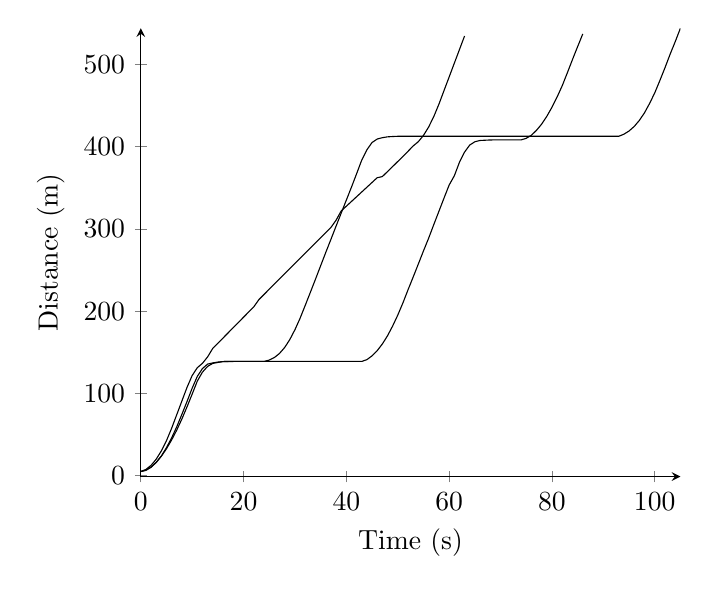
\begin{tikzpicture}
\begin{axis}[
legend style={
	anchor=west
},
axis x line=bottom,
axis y line=left,
ymin=-1,
point meta=explicit symbolic,
xlabel=Time (s),
ylabel=Distance (m)
]
\addplot[] coordinates {
(0, 5.1)
(1, 7.6)
(2, 12.6)
(3, 20.1)
(4, 30.1)
(5, 42.6)
(6, 57.6)
(7, 74.2)
(8, 90.8)
(9, 107.4)
(10, 121.758781889)
(11, 131.320742477)
(12, 136.609280481)
(13, 144.397818486)
(14, 154.68635649)
(15, 161.021784205)
(16, 167.357487819)
(17, 173.693488531)
(18, 180.029809771)
(19, 186.366477498)
(20, 192.703520555)
(21, 199.040971076)
(22, 205.378864977)
(23, 214.216758878)
(24, 220.474798436)
(25, 226.732975077)
(26, 232.991302485)
(27, 239.24979623)
(28, 245.508474103)
(29, 251.76735653)
(30, 258.026467073)
(31, 264.285833063)
(32, 270.54548638)
(33, 276.805464446)
(34, 283.065811483)
(35, 289.326580132)
(36, 295.58783356)
(37, 301.849648237)
(38, 310.611462913)
(39, 321.873277589)
(40, 327.639455454)
(41, 333.40702523)
(42, 339.176282693)
(43, 344.947614137)
(44, 350.721534016)
(45, 356.498743209)
(46, 362.280222462)
(47, 363.607388781)
(48, 369.687974655)
(49, 375.790220913)
(50, 381.925195852)
(51, 388.113297227)
(52, 394.397230867)
(53, 400.887229602)
(54, 406.011673174)
(55, 413.636116745)
(56, 423.760560316)
(57, 436.385003888)
(58, 451.509447459)
(59, 468.109447459)
(60, 484.709447459)
(61, 501.309447459)
(62, 517.909447459)
(63, 534.509447459)
};
\addplot[] coordinates {
(0, 5.1)
(1, 6.72319098396)
(2, 10.3468733498)
(3, 16.1332685505)
(4, 23.9286882805)
(5, 34.1720166711)
(6, 45.8890593831)
(7, 59.528275984)
(8, 74.6547246313)
(9, 90.2617056908)
(10, 106.406079189)
(11, 120.752868035)
(12, 130.281439818)
(13, 135.692922631)
(14, 137.147873208)
(15, 138.151456947)
(16, 138.752549833)
(17, 138.919508134)
(18, 138.930273837)
(19, 138.930273837)
(20, 138.930273837)
(21, 138.930273837)
(22, 138.930273837)
(23, 138.930273837)
(24, 138.930273837)
(25, 138.930273837)
(26, 138.930273837)
(27, 138.930273837)
(28, 138.930273837)
(29, 138.930273837)
(30, 138.930273837)
(31, 138.930273837)
(32, 138.930273837)
(33, 138.930273837)
(34, 138.930273837)
(35, 138.930273837)
(36, 138.930273837)
(37, 138.930273837)
(38, 138.930273837)
(39, 138.930273837)
(40, 138.930273837)
(41, 138.930273837)
(42, 138.930273837)
(43, 138.930273837)
(44, 141.114915808)
(45, 145.723578326)
(46, 151.998746932)
(47, 160.122800526)
(48, 170.022035583)
(49, 181.88207967)
(50, 195.182643297)
(51, 209.951444677)
(52, 226.009298917)
(53, 241.535058473)
(54, 257.259677345)
(55, 273.192092192)
(56, 288.571607169)
(57, 305.072725588)
(58, 321.279140443)
(59, 337.433303376)
(60, 353.346931963)
(61, 364.463502929)
(62, 380.895988341)
(63, 393.376922659)
(64, 401.949110189)
(65, 405.94426858)
(66, 407.522011955)
(67, 407.847468212)
(68, 408.163202868)
(69, 408.195381563)
(70, 408.195381563)
(71, 408.195381563)
(72, 408.195381563)
(73, 408.195381563)
(74, 408.195381563)
(75, 410.18501972)
(76, 413.845617016)
(77, 419.917654902)
(78, 427.393386755)
(79, 436.836262111)
(80, 447.819760421)
(81, 460.280904293)
(82, 474.035882427)
(83, 489.7969413)
(84, 505.936939978)
(85, 521.577093631)
(86, 537.018117137)
};
\addplot[] coordinates {
(0, 5.1)
(1, 6.52942920473)
(2, 10.397460774)
(3, 16.2332625509)
(4, 23.6898428533)
(5, 32.7746166262)
(6, 43.4439596056)
(7, 55.4796695473)
(8, 68.9530208007)
(9, 83.7525044986)
(10, 99.1987196739)
(11, 115.018047915)
(12, 125.904988034)
(13, 132.893465407)
(14, 136.539717246)
(15, 137.713754698)
(16, 138.775338083)
(17, 138.887378187)
(18, 138.919642787)
(19, 138.937871182)
(20, 138.937871182)
(21, 138.937871182)
(22, 138.937871182)
(23, 138.937871182)
(24, 138.937871182)
(25, 140.600580891)
(26, 143.690544118)
(27, 148.673520683)
(28, 155.907791651)
(29, 165.526496226)
(30, 177.544292589)
(31, 191.406263769)
(32, 207.110921725)
(33, 222.961991482)
(34, 239.000783121)
(35, 255.251148179)
(36, 271.513491617)
(37, 287.341622586)
(38, 303.408023612)
(39, 319.255356152)
(40, 335.112647816)
(41, 350.841227009)
(42, 367.19319554)
(43, 383.738226039)
(44, 396.198486332)
(45, 405.06887588)
(46, 409.280332872)
(47, 410.942766083)
(48, 411.946804448)
(49, 412.338587013)
(50, 412.617241737)
(51, 412.658060886)
(52, 412.658060886)
(53, 412.658060886)
(54, 412.658060886)
(55, 412.658060886)
(56, 412.658060886)
(57, 412.658060886)
(58, 412.658060886)
(59, 412.658060886)
(60, 412.658060886)
(61, 412.658060886)
(62, 412.658060886)
(63, 412.658060886)
(64, 412.658060886)
(65, 412.658060886)
(66, 412.658060886)
(67, 412.658060886)
(68, 412.658060886)
(69, 412.658060886)
(70, 412.658060886)
(71, 412.658060886)
(72, 412.658060886)
(73, 412.658060886)
(74, 412.658060886)
(75, 412.658060886)
(76, 412.658060886)
(77, 412.658060886)
(78, 412.658060886)
(79, 412.658060886)
(80, 412.658060886)
(81, 412.658060886)
(82, 412.658060886)
(83, 412.658060886)
(84, 412.658060886)
(85, 412.658060886)
(86, 412.658060886)
(87, 412.658060886)
(88, 412.658060886)
(89, 412.658060886)
(90, 412.658060886)
(91, 412.658060886)
(92, 412.658060886)
(93, 412.658060886)
(94, 415.153000888)
(95, 419.023672137)
(96, 424.501100973)
(97, 431.86335141)
(98, 441.039908442)
(99, 452.511470428)
(100, 465.308069565)
(101, 480.38143179)
(102, 496.032202461)
(103, 512.437839659)
(104, 527.797351639)
(105, 543.987083911)
};

\end{axis}
\end{tikzpicture}
\label{tik:50:12_O, 13_S, 15_N, 17_S, 17_S.-60, 19_V}
\caption{50 percent diving with GSC on route $12_O, 13_S, 15_N, 17_S, 17_S.-60, 19_V$}
\end{figure}

%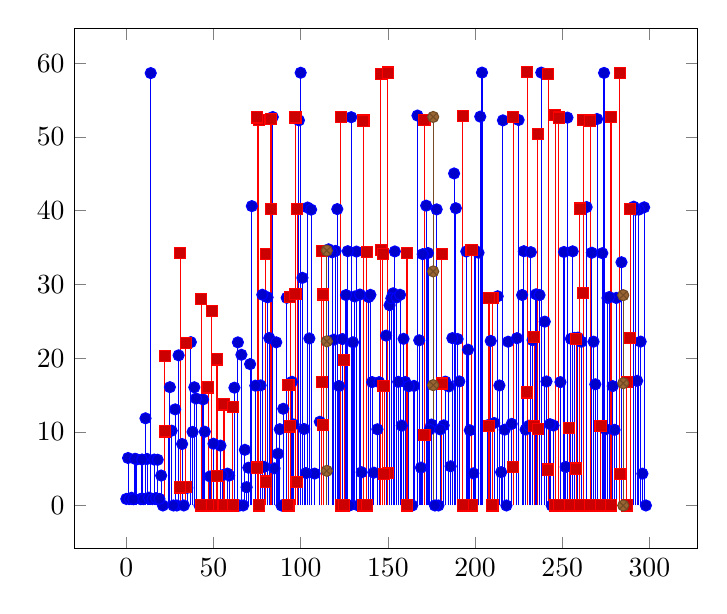
\begin{tikzpicture}\begin{axis} [width=9.5cm]
\addplot+[ycomb] coordinates{
(216, 52.252945617)
(217, 10.2835247016)
(214, 16.2856718575)
(215, 4.51864792679)
(213, 28.3873548357)
(211, 11.189338998)
(264, 40.4878802965)
(218, 0)
(219, 22.2220848566)
(133, 0)
(132, 34.4508958132)
(131, 28.3594198907)
(130, 22.1385166496)
(137, 0)
(135, 4.50616611369)
(165, 16.2267027888)
(139, 28.285187868)
(225, 52.3061097447)
(25, 16.0530002679)
(26, 10.1475132786)
(167, 52.905635371)
(20, 4.06070836139)
(21, 0)
(95, 16.7780005237)
(28, 13.0397800766)
(29, 0)
(178, 40.1749084596)
(0, 0.887926285604)
(221, 11.0667215168)
(281, 28.1590830651)
(8, 0.879701275233)
(96, 10.9849476286)
(284, 33.0003184931)
(68, 7.55165507934)
(87, 7.01750211778)
(119, 22.4988880985)
(263, 0)
(121, 40.2128463437)
(261, 22.2161474214)
(124, 22.5816882433)
(265, 0)
(127, 34.5048855528)
(128, 0)
(129, 52.6828088003)
(269, 16.4398851063)
(268, 22.2261723856)
(183, 16.8024845352)
(59, 4.06105996166)
(58, 4.32362219439)
(55, 4.10269772145)
(54, 8.12141482104)
(227, 28.5551151413)
(50, 8.38010669551)
(53, 0)
(259, 22.7745844792)
(298, 0)
(296, 4.31694972892)
(297, 40.4553565181)
(294, 40.1480987865)
(295, 22.2334499586)
(292, 40.1264458833)
(293, 16.9100041831)
(291, 40.5409654352)
(199, 4.35555745706)
(66, 20.4512404622)
(134, 28.6189430663)
(194, 0)
(197, 10.2047254435)
(196, 21.1414626766)
(191, 16.8319208832)
(190, 22.5846717422)
(271, 0)
(273, 34.2295001485)
(111, 11.3590799416)
(275, 10.3466370086)
(276, 28.1627318956)
(82, 22.718673814)
(279, 16.198959792)
(81, 28.2427318469)
(86, 22.1371668922)
(175, 10.9783281237)
(84, 52.7044109674)
(85, 5.04021199249)
(251, 34.3955366687)
(140, 28.580112231)
(108, 4.326167767)
(173, 34.2552838173)
(141, 16.7396435688)
(172, 40.6837062669)
(27, 0)
(3, 1.04420549155)
(255, 22.6172191574)
(24, 10.0531682208)
(245, 10.8464242737)
(244, 0)
(247, 0)
(241, 16.8271854495)
(240, 24.9439593649)
(243, 11.0294469892)
(102, 10.3777836793)
(103, 4.39269776309)
(100, 58.715030228)
(101, 30.8873579857)
(249, 16.738667879)
(104, 40.4248832298)
(105, 22.6658469812)
(39, 16.0389462527)
(38, 9.97543373366)
(33, 0)
(32, 8.33961614558)
(224, 22.6943008186)
(30, 20.3718391591)
(37, 22.1587029266)
(35, 2.38991943591)
(252, 5.22601443101)
(64, 22.13130224)
(65, 0)
(179, 0)
(67, 0)
(177, 0)
(69, 2.47903564849)
(174, 10.3127546711)
(256, 34.4823477755)
(257, 22.7308631355)
(170, 34.098783136)
(203, 52.7582624606)
(253, 52.6262542806)
(182, 10.8682501666)
(195, 34.4655481847)
(180, 10.3224731989)
(2, 0.889785751671)
(186, 5.31367419411)
(187, 22.7052298423)
(185, 16.1605886549)
(188, 45.0508173792)
(189, 40.3306851983)
(202, 34.2922024545)
(4, 0.858119596325)
(120, 34.5436475256)
(6, 6.26091222826)
(57, 0)
(99, 52.2575951587)
(168, 22.4135028295)
(169, 5.13775554004)
(229, 10.295455161)
(228, 34.5018262923)
(164, 0)
(92, 28.1764589812)
(160, 16.7564116485)
(162, 16.1825565598)
(11, 11.8283948176)
(10, 0.881112011558)
(13, 1.06146657052)
(12, 6.31020600882)
(15, 0.875296659051)
(14, 58.6672268685)
(17, 0.993840898557)
(16, 6.22794134696)
(19, 0.888781204593)
(18, 6.20293203127)
(118, 34.3543907429)
(88, 10.34819743)
(116, 34.7586327154)
(274, 58.6919651903)
(151, 27.1786828977)
(153, 28.7878919466)
(152, 28.1038034905)
(155, 28.2228618291)
(154, 34.4696486913)
(157, 28.5873349819)
(156, 16.775155837)
(159, 22.6084045705)
(158, 10.8361840758)
(62, 15.9833105543)
(277, 28.2764304681)
(90, 13.1217001857)
(238, 58.7327045428)
(235, 28.6501799394)
(237, 28.5527321263)
(231, 10.8267935469)
(232, 34.3695501862)
(233, 22.445048936)
(280, 10.2601636215)
(48, 3.93928596866)
(46, 0)
(44, 14.3903646534)
(45, 10.0088845232)
(42, 0)
(40, 14.5185355396)
(1, 6.44158771882)
(5, 6.33155562465)
(9, 6.23692159842)
(200, 34.5846228307)
(144, 10.3377609298)
(145, 16.728360112)
(142, 4.4518685762)
(204, 58.7375726484)
(207, 10.8693114242)
(209, 22.3262391201)
(149, 23.0494155894)
(77, 16.2953052439)
(74, 16.2546317465)
(106, 40.1412078513)
(72, 40.6167688582)
(71, 19.1793620961)
(70, 5.12135647663)
(79, 5.24282483604)
(78, 28.596095633)
(122, 16.2074955811)
(270, 52.4359425241)
(89, 0)
(267, 34.2918595684)
(126, 28.5503390242)};
\addplot+[ycomb] coordinates{
(210, 28.1097793763)
(210, 0)
(136, 52.2280479547)
(136, 0)
(138, 34.3467427786)
(138, 0)
(198, 34.6152811937)
(198, 0)
(22, 20.3266947089)
(22, 10.0447349346)
(289, 40.1976509476)
(289, 22.7168289734)
(283, 58.6320978831)
(283, 4.31438946042)
(123, 52.7292763657)
(123, 0)
(125, 19.7400405749)
(125, 0)
(56, 13.7112306443)
(56, 0)
(52, 19.8176908191)
(52, 4.04307309312)
(146, 58.5827933491)
(146, 34.6907037185)
(147, 34.1110400653)
(147, 16.2145455372)
(193, 52.8336680281)
(193, 0)
(80, 34.1002985828)
(80, 3.24308949069)
(254, 10.5251603275)
(254, 0)
(242, 58.5806667528)
(242, 4.87870006484)
(161, 34.2151874165)
(161, 0)
(34, 22.0585066331)
(34, 2.49293574307)
(246, 53.011035511)
(246, 0)
(94, 28.2491635302)
(94, 10.727029223)
(61, 13.312000988)
(61, 0)
(258, 22.6217152778)
(258, 5.01039621943)
(171, 52.3163917096)
(171, 9.55366723979)
(272, 10.8338464926)
(272, 0)
(181, 34.151374051)
(181, 16.5489447218)
(248, 52.6363940379)
(248, 0)
(97, 52.6547729656)
(97, 28.6648254432)
(98, 40.2593862116)
(98, 3.21946066682)
(222, 52.6819066117)
(222, 5.23552143383)
(93, 16.3158568778)
(93, 0)
(287, 16.7670833498)
(287, 0)
(31, 34.255056387)
(31, 2.44722481145)
(150, 58.7435786763)
(150, 4.41595408894)
(113, 28.6293422449)
(113, 10.9734549893)
(278, 52.6666260662)
(278, 0)
(83, 52.4478526303)
(83, 40.1971805753)
(234, 22.8473160709)
(234, 10.8390960135)
(236, 50.4031601251)
(236, 10.3285979681)
(230, 58.8696240113)
(230, 15.341659667)
(49, 26.3558240891)
(49, 0)
(47, 16.0158863142)
(47, 0)
(43, 27.9870688156)
(43, 0)
(208, 28.1330483343)
(208, 10.7370070602)
(148, 16.2311692676)
(148, 4.29963387855)
(76, 52.2595937482)
(76, 0)
(75, 52.6464795668)
(75, 5.15014459374)
(112, 34.4737051594)
(112, 16.80717737)
(262, 52.3174756198)
(262, 28.7833548519)
(260, 40.2876209009)
(260, 0)
(266, 52.2325690044)
(266, 0)};
\addplot+[ycomb] coordinates{
(285, 28.5350456998)
(285, 16.5886687888)
(285, 0)
(115, 34.5913828471)
(115, 22.27329098)
(115, 4.69795317646)
(176, 52.7187685594)
(176, 31.7604481719)
(176, 16.3285637619)
};
\end{axis}\end{tikzpicture}

\subsection{Fuel Consumption}
The purpose of \tech is to reduce fuel consumption. 
We use SUMO's build-in function to calculate the vehicles fuel consumption, which is explained in \cite{SUMOFuel}.

%Figure~\ref{tik:fuel:0:51} shows this fuel consumption as a function of time for vehicles driving on route 51 controlled by SUMO only. 
%Figure~\ref{tik:fuel:100:51} shows the same setup, but with all vehicles controlled by \tech.
Figure~\ref{fig:TestResults:fuelRoute} plots the average fuel consumption for vehicles driving on all routes. 
The results clearly show that using \tech in this setup will reduce the fuel consumption significantly.
Acrose all routes, we see a reduction from an average of 130 $mL$ to an average of 96 $mL$, which is a reduction of 29 \%.
If we only look at route 1, we observe an average fuel consumption without \tech at 175 $mL$, and 117 $mL$ with \tech.
This is again a significant reduction in fuel consumption in 33 \%. %TODO fix number

\begin{figure}[htb]
\includegraphics[width=0.5\textwidth]{images/tp0/fuelRoute.png}
\caption{Fuel graph}
\label{fig:TestResults:fuelRoute}
\end{figure}


%
\begin{figure}
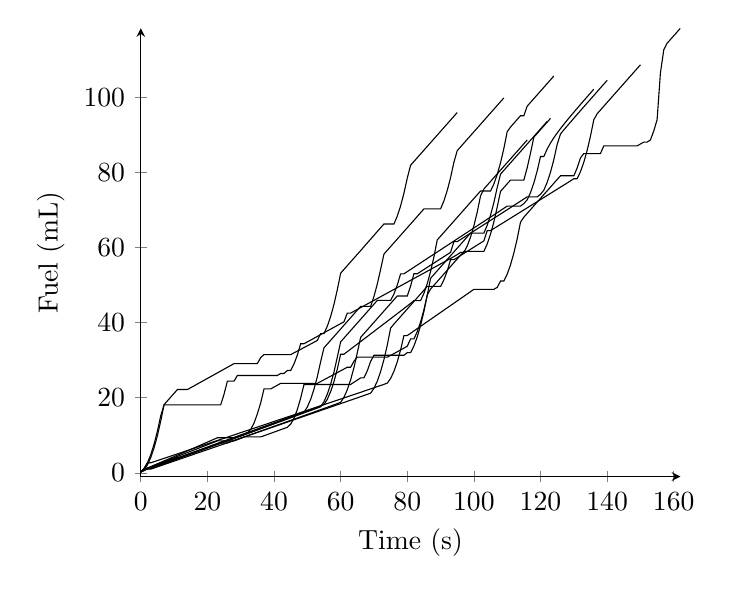
\begin{tikzpicture}
\begin{axis}[
legend style={anchor=west},
axis x line=bottom,
axis y line=left,
ymin=-1,
xlabel=Time (s),
ylabel=Fuel (mL),
]
\addplot[] coordinates {
(0, 0.239885513361)
(1, 0.766617621116)
(2, 1.08709758181)
(3, 1.40758497837)
(4, 1.72808020027)
(5, 2.04858366472)
(6, 2.36909581918)
(7, 2.68961714422)
(8, 3.01014815659)
(9, 3.33068941274)
(10, 3.6512415127)
(11, 3.97180510443)
(12, 4.29238088878)
(13, 4.61296962496)
(14, 4.93357213677)
(15, 5.25418931972)
(16, 5.57482214894)
(17, 5.89547168835)
(18, 6.21613910102)
(19, 6.53682566105)
(20, 6.85753276724)
(21, 7.17826195881)
(22, 7.49901493359)
(23, 7.81979356912)
(24, 8.14059994722)
(25, 8.46143638284)
(26, 8.78230545781)
(27, 9.10453591631)
(28, 9.4276709852)
(29, 9.75116298729)
(30, 10.0737554582)
(31, 10.3963723276)
(32, 10.7190161515)
(33, 11.04168986)
(34, 11.3643968287)
(35, 11.6871409684)
(36, 12.0099268366)
(37, 12.3327597795)
(38, 12.655646113)
(39, 12.978593358)
(40, 13.3016105483)
(41, 13.6247086404)
(42, 13.9479010682)
(43, 14.2712045075)
(44, 14.5946399521)
(45, 14.918234265)
(46, 15.2420224816)
(47, 15.5660513463)
(48, 15.8903849693)
(49, 16.2151143487)
(50, 16.5403744605)
(51, 16.8663776308)
(52, 17.1934867013)
(53, 17.522405092)
(54, 17.8548280695)
(55, 18.1973707627)
(56, 19.595563849)
(57, 21.6312611565)
(58, 24.3053215731)
(59, 27.6250572516)
(60, 31.6042336095)
(61, 31.6042336095)
(62, 32.2792361189)
(63, 32.9542416009)
(64, 33.6292505828)
(65, 34.3042637193)
(66, 34.9792818336)
(67, 35.6543059721)
(68, 36.3293374845)
(69, 37.0043781377)
(70, 37.6794302852)
(71, 38.3544971234)
(72, 39.029583091)
(73, 39.7046945116)
(74, 40.3798406682)
(75, 41.0557239752)
(76, 41.732784354)
(77, 42.4108338501)
(78, 43.0904833237)
(79, 43.7729239316)
(80, 44.4607689175)
(81, 45.1608350129)
(82, 45.8944650363)
(83, 45.8944650363)
(84, 45.8944650363)
(85, 47.8396063179)
(86, 50.422594991)
(87, 53.6498255499)
(88, 57.534145754)
(89, 62.0576642363)
(90, 63.0616540993)
(91, 64.0656439623)
(92, 65.0696338253)
(93, 66.0736236884)
(94, 67.0776135514)
(95, 68.0816034144)
(96, 69.0855932774)
(97, 70.0895831405)
(98, 71.0935730035)
(99, 72.0975628665)
(100, 73.1015527295)
(101, 74.1055425925)
(102, 75.1095324556)
(103, 75.1095324556)
(104, 75.1095324556)
(105, 75.1095324556)
(106, 76.978263322)
(107, 79.4845079301)
(108, 82.6338864636)
(109, 86.4384723714)
(110, 90.9167923671)
(111, 92.1580150926)
(112, 93.1620049556)
(113, 94.1659948186)
(114, 95.1699846817)
(115, 95.1699846817)
(116, 97.7152725592)
(117, 98.7192624222)
(118, 99.7232522853)
(119, 100.727242148)
(120, 101.731232011)
(121, 102.735221874)
(122, 103.739211737)
(123, 104.7432016)
(124, 105.747191463)
};
\addplot[] coordinates {
(0, 0.239885513361)
(1, 0.721796247693)
(2, 1.0358082283)
(3, 1.34982637617)
(4, 1.66385098473)
(5, 1.97788236635)
(6, 2.29192085391)
(7, 2.60596680255)
(8, 2.92002059156)
(9, 3.23408262644)
(10, 3.54815334123)
(11, 3.8622332011)
(12, 4.17632270518)
(13, 4.49042238972)
(14, 4.80453283163)
(15, 5.11865465244)
(16, 5.43278852269)
(17, 5.74693516691)
(18, 6.06109536916)
(19, 6.37526997933)
(20, 6.68945992023)
(21, 7.0036661956)
(22, 7.31788989928)
(23, 7.63213222558)
(24, 7.94639448118)
(25, 7.94639448118)
(26, 7.94639448118)
(27, 8.27747161143)
(28, 8.59219066325)
(29, 8.90742530016)
(30, 9.22370449251)
(31, 9.54064186901)
(32, 9.85737353126)
(33, 10.1737064241)
(34, 10.4900600247)
(35, 10.8064363194)
(36, 11.1228375603)
(37, 11.4392663111)
(38, 11.7557255038)
(39, 12.072218509)
(40, 12.3887492212)
(41, 12.7053221678)
(42, 13.0219426446)
(43, 13.3386168902)
(44, 13.6553523102)
(45, 13.9721577711)
(46, 14.2890439889)
(47, 14.6060240543)
(48, 14.9231141531)
(49, 15.2403345763)
(50, 15.5577111711)
(51, 15.8752774856)
(52, 16.1930780482)
(53, 16.5111735901)
(54, 16.8296497965)
(55, 17.1486329395)
(56, 17.4683202589)
(57, 17.7890462403)
(58, 18.11145389)
(59, 18.4370782708)
(60, 18.7718404678)
(61, 20.132860248)
(62, 22.131532813)
(63, 24.7683418673)
(64, 28.0502243804)
(65, 31.9905705868)
(66, 36.0839399334)
(67, 37.0879297965)
(68, 38.0919196595)
(69, 39.0959095225)
(70, 40.0998993855)
(71, 41.1038892486)
(72, 42.1078791116)
(73, 43.1118689746)
(74, 44.1158588376)
(75, 45.1198487006)
(76, 46.1238385637)
(77, 47.1278284267)
(78, 47.1278284267)
(79, 47.1278284267)
(80, 47.1278284267)
(81, 49.7619304093)
(82, 53.041062953)
(83, 53.041062953)
(84, 53.6124281296)
(85, 54.1837933355)
(86, 54.7551585738)
(87, 55.3265238478)
(88, 55.8978891615)
(89, 56.4692545192)
(90, 57.0406742607)
(91, 57.6120547424)
(92, 58.1834268074)
(93, 58.754798918)
(94, 61.6018599133)
(95, 61.6018599133)
(96, 62.1690141416)
(97, 62.7361859918)
(98, 63.3033783496)
(99, 63.8705947484)
(100, 64.4378395577)
(101, 65.0051182398)
(102, 65.5724377052)
(103, 66.1398068138)
(104, 66.7072370948)
(105, 67.2747438028)
(106, 67.8423475078)
(107, 68.4100765519)
(108, 68.9779709701)
(109, 69.5460889807)
(110, 70.1145181976)
(111, 70.6833960192)
(112, 71.2529490718)
(113, 71.8235756346)
(114, 72.3954060082)
(115, 72.9721206516)
(116, 73.555576238)
(117, 73.555576238)
(118, 73.555576238)
(119, 73.555576238)
(120, 74.2240216111)
(121, 75.3210347799)
(122, 77.398241346)
(123, 80.1140910005)
(124, 83.4763164865)
(125, 87.4991038124)
(126, 90.3186177379)
(127, 91.3829197557)
(128, 92.4304792154)
(129, 93.4660854342)
(130, 94.4930927181)
(131, 95.5138796674)
(132, 96.5301485974)
(133, 97.5431261577)
(134, 98.5537007135)
(135, 99.5625180369)
(136, 100.570048844)
(137, 101.576636944)
(138, 102.582533827)
(139, 103.587923657)
(140, 104.596899343)
};
\addplot[] coordinates {
(0, 0.239885513361)
(1, 0.841669203293)
(2, 1.17158097305)
(3, 1.50150231265)
(4, 1.83143379257)
(5, 2.16137602963)
(6, 2.49132969183)
(7, 2.82129550378)
(8, 3.15127425287)
(9, 3.48126679619)
(10, 3.81127406847)
(11, 4.14129709111)
(12, 4.14129709111)
(13, 4.47093324678)
(14, 4.80057872468)
(15, 5.130234237)
(16, 5.45990057065)
(17, 5.78957859733)
(18, 6.11926928537)
(19, 6.44897371352)
(20, 6.77869308723)
(21, 7.10842875797)
(22, 7.43818224613)
(23, 7.76795526841)
(24, 8.09903345715)
(25, 8.43193196978)
(26, 8.43193196978)
(27, 8.78943402268)
(28, 9.12186908749)
(29, 9.45431543139)
(30, 9.78677447663)
(31, 10.1192478976)
(32, 10.4517376797)
(33, 10.7842461966)
(34, 11.1167763109)
(35, 11.4493315094)
(36, 11.7819160864)
(37, 12.114535397)
(38, 12.4471962146)
(39, 12.7799072486)
(40, 13.1126799133)
(41, 13.4455295114)
(42, 13.7784771269)
(43, 14.1115528111)
(44, 14.4448012843)
(45, 14.7782930166)
(46, 15.1121483137)
(47, 15.4465990161)
(48, 15.7821949679)
(49, 16.1209905479)
(50, 17.5334240011)
(51, 19.5833105246)
(52, 22.2716527829)
(53, 25.6059067053)
(54, 29.5999814862)
(55, 33.3061568052)
(56, 34.3101466682)
(57, 35.3141365312)
(58, 36.3181263943)
(59, 37.3221162573)
(60, 38.3261061203)
(61, 39.3300959833)
(62, 40.3340858463)
(63, 41.3380757094)
(64, 42.3420655724)
(65, 43.3460554354)
(66, 44.3500452984)
(67, 44.3500452984)
(68, 44.3500452984)
(69, 44.3500452984)
(70, 46.9911366921)
(71, 50.2773696364)
(72, 54.2221775082)
(73, 58.282460115)
(74, 59.2864499781)
(75, 60.2904398411)
(76, 61.2944297041)
(77, 62.2984195671)
(78, 63.3024094302)
(79, 64.3063992932)
(80, 65.3103891562)
(81, 66.3143790192)
(82, 67.3183688823)
(83, 68.3223587453)
(84, 69.3263486083)
(85, 70.3303384713)
(86, 70.3303384713)
(87, 70.3303384713)
(88, 70.3303384713)
(89, 70.3303384713)
(90, 70.3303384713)
(91, 72.4648003665)
(92, 75.2383364436)
(93, 78.659259489)
(94, 82.7423355536)
(95, 85.8598887676)
(96, 86.8638786306)
(97, 87.8678684936)
(98, 88.8718583566)
(99, 89.8758482197)
(100, 90.8798380827)
(101, 91.8838279457)
(102, 92.8878178087)
(103, 93.8918076718)
(104, 94.8957975348)
(105, 95.8997873978)
(106, 96.9037772608)
(107, 97.9077671239)
(108, 98.9117569869)
(109, 99.9157468499)
};
\addplot[] coordinates {
(0, 0.239885513361)
(1, 1.13183007041)
(2, 2.66515136892)
(3, 2.66515136892)
(4, 2.96235257606)
(5, 3.25955820712)
(6, 3.55676843281)
(7, 3.85398343273)
(8, 4.15120339604)
(9, 4.44842852202)
(10, 4.74565902083)
(11, 5.04289511423)
(12, 5.34013703641)
(13, 5.63738503487)
(14, 5.93463937137)
(15, 6.23190032301)
(16, 6.52916818334)
(17, 6.82644326363)
(18, 7.12372589422)
(19, 7.42101642604)
(20, 7.71831523218)
(21, 8.01562270977)
(22, 8.31293928188)
(23, 8.61026539973)
(24, 8.90760154507)
(25, 9.20494823284)
(26, 9.50230601407)
(27, 9.79967547914)
(28, 10.0970572614)
(29, 10.3944520411)
(30, 10.6918605499)
(31, 10.9892835761)
(32, 11.2867219696)
(33, 11.584487037)
(34, 11.8827476291)
(35, 12.1813654198)
(36, 12.480364028)
(37, 12.7791215077)
(38, 13.0778021433)
(39, 13.3764940493)
(40, 13.675198016)
(41, 13.9739149096)
(42, 14.2726456827)
(43, 14.5713913849)
(44, 14.8701531758)
(45, 15.1689323401)
(46, 15.4677303049)
(47, 15.7665486608)
(48, 16.0653891859)
(49, 16.3642538755)
(50, 16.6631449759)
(51, 16.9620650271)
(52, 17.2610169129)
(53, 17.5600039227)
(54, 17.8590298276)
(55, 18.1580989739)
(56, 18.4572164013)
(57, 18.7563879913)
(58, 19.0556206571)
(59, 19.3549225898)
(60, 19.6543035811)
(61, 19.9537754542)
(62, 20.2533526483)
(63, 20.5530530291)
(64, 20.8528990394)
(65, 21.15291938)
(66, 21.4531515465)
(67, 21.7536458203)
(68, 22.0544718671)
(69, 22.3557303682)
(70, 22.6575753117)
(71, 22.9602619193)
(72, 23.2642685836)
(73, 23.5707050723)
(74, 23.8837013296)
(75, 25.1400136243)
(76, 27.0345137512)
(77, 29.5666297562)
(78, 32.7422429499)
(79, 36.5736879078)
(80, 36.5736879078)
(81, 37.1894854606)
(82, 37.8052847332)
(83, 38.4210859741)
(84, 39.0368894804)
(85, 39.6526956109)
(86, 40.2685048014)
(87, 40.8843175871)
(88, 41.5001346311)
(89, 42.1159567648)
(90, 42.7317850424)
(91, 43.3476208197)
(92, 43.963465866)
(93, 44.5793225301)
(94, 45.1951939904)
(95, 45.8110846423)
(96, 46.4270364848)
(97, 47.0439221787)
(98, 47.6612467951)
(99, 48.2792081915)
(100, 48.89813525)
(101, 48.89813525)
(102, 48.89813525)
(103, 48.89813525)
(104, 48.89813525)
(105, 48.89813525)
(106, 48.89813525)
(107, 49.4127215327)
(108, 51.1084813475)
(109, 51.1084813475)
(110, 52.9547626197)
(111, 55.4384772704)
(112, 58.5650180069)
(113, 62.3462308016)
(114, 66.8004148913)
(115, 68.1235435499)
(116, 69.1275334129)
(117, 70.131523276)
(118, 71.135513139)
(119, 72.139503002)
(120, 73.143492865)
(121, 74.1474827281)
(122, 75.1514725911)
(123, 76.1554624541)
(124, 77.1594523171)
(125, 78.1634421802)
(126, 79.1674320432)
(127, 79.1674320432)
(128, 79.1674320432)
(129, 79.1674320432)
(130, 79.1674320432)
(131, 81.2350104653)
(132, 83.9411645953)
(133, 85.0856655006)
(134, 85.0856655006)
(135, 85.0856655006)
(136, 85.0856655006)
(137, 85.0856655006)
(138, 85.0856655006)
(139, 87.1302386009)
(140, 87.1302386009)
(141, 87.1302386009)
(142, 87.1302386009)
(143, 87.1302386009)
(144, 87.1302386009)
(145, 87.1302386009)
(146, 87.1302386009)
(147, 87.1302386009)
(148, 87.1302386009)
(149, 87.1302386009)
(150, 87.6344866857)
(151, 88.1387810755)
(152, 88.1387810755)
(153, 88.7285525069)
(154, 91.1042606744)
(155, 94.1214294934)
(156, 106.573118119)
(157, 112.70473431)
(158, 114.476541069)
(159, 115.480530932)
(160, 116.484520795)
(161, 117.488510658)
(162, 118.492500521)
};
\addplot[] coordinates {
(0, 0.239885513361)
(1, 0.670769182584)
(2, 0.97634956868)
(3, 0.97634956868)
(4, 1.28173702068)
(5, 1.58712693446)
(6, 1.89251941507)
(7, 2.19791457363)
(8, 2.5033125278)
(9, 2.80871340223)
(10, 3.11411732915)
(11, 3.4195244489)
(12, 3.72493491058)
(13, 4.03034887276)
(14, 4.33576650425)
(15, 4.64118798492)
(16, 4.94661350664)
(17, 5.25204327429)
(18, 5.5574775069)
(19, 5.86291643891)
(20, 6.16836032151)
(21, 6.47380942422)
(22, 6.77926403658)
(23, 7.08472447004)
(24, 7.39019106012)
(25, 7.69566416876)
(26, 8.001144187)
(27, 8.30663153799)
(28, 8.61212668037)
(29, 8.9176301121)
(30, 9.22314237479)
(31, 9.52866405863)
(32, 9.83419580801)
(33, 10.1405566481)
(34, 10.4475696363)
(35, 10.7551515939)
(36, 11.0626101217)
(37, 11.3697363697)
(38, 11.6768674172)
(39, 11.9840036593)
(40, 12.2911455359)
(41, 12.5982935385)
(42, 12.9054482185)
(43, 13.2126101959)
(44, 13.5197801716)
(45, 13.8269589402)
(46, 14.1341474068)
(47, 14.4413466077)
(48, 14.7485577349)
(49, 15.0557821674)
(50, 15.3630215103)
(51, 15.6702776442)
(52, 15.9775527885)
(53, 16.2848495839)
(54, 16.5921712007)
(55, 16.8995214837)
(56, 17.206905149)
(57, 17.5143280581)
(58, 17.8217976068)
(59, 18.1293232937)
(60, 18.4369175789)
(61, 18.7445972328)
(62, 19.0523855609)
(63, 19.3603163109)
(64, 19.6684411138)
(65, 19.9768453387)
(66, 20.2856878897)
(67, 20.5953316392)
(68, 20.9070759547)
(69, 21.2222070277)
(70, 22.5016131427)
(71, 24.4190743231)
(72, 26.9742512933)
(73, 30.1732580424)
(74, 34.0286618246)
(75, 38.5594831588)
(76, 39.6365881465)
(77, 40.6405780095)
(78, 41.6445678725)
(79, 42.6485577356)
(80, 43.6525475986)
(81, 44.6565374616)
(82, 45.6605273246)
(83, 46.6645171877)
(84, 47.6685070507)
(85, 48.6724969137)
(86, 49.6764867767)
(87, 49.6764867767)
(88, 49.6764867767)
(89, 49.6764867767)
(90, 49.6764867767)
(91, 51.413532691)
(92, 53.7877354245)
(93, 56.8033810707)
(94, 56.8033810707)
(95, 57.3587054684)
(96, 57.914030616)
(97, 58.4693565872)
(98, 59.0246834657)
(99, 59.5800113466)
(100, 60.1353403387)
(101, 60.6907425922)
(102, 61.2460821515)
(103, 61.8014232753)
(104, 64.5476058339)
(105, 64.5476058339)
(106, 65.0990555305)
(107, 65.650508463)
(108, 66.2019651102)
(109, 66.7534260481)
(110, 67.3048919746)
(111, 67.8563637437)
(112, 68.4078424104)
(113, 68.9593292917)
(114, 69.5108260517)
(115, 70.0623348211)
(116, 70.6138583682)
(117, 71.1654003496)
(118, 71.716965687)
(119, 72.2685611476)
(120, 72.8201962676)
(121, 73.371884877)
(122, 73.9236477226)
(123, 74.4755172155)
(124, 75.0275465627)
(125, 75.5798287059)
(126, 76.1324848557)
(127, 76.6859794371)
(128, 77.2411791602)
(129, 77.8009731661)
(130, 78.3807087889)
(131, 78.3807087889)
(132, 80.2519865043)
(133, 82.760787585)
(134, 85.9127580223)
(135, 89.7199970722)
(136, 94.1021001543)
(137, 95.6943595191)
(138, 96.6983493821)
(139, 97.7023392451)
(140, 98.7063291081)
(141, 99.7103189712)
(142, 100.714308834)
(143, 101.718298697)
(144, 102.72228856)
(145, 103.726278423)
(146, 104.730268286)
(147, 105.734258149)
(148, 106.738248012)
(149, 107.742237875)
(150, 108.746227738)
};
\addplot[] coordinates {
(0, 0.239885513361)
(1, 0.777249275829)
(2, 1.09916109643)
(3, 1.09916109643)
(4, 1.42083073583)
(5, 1.74250449665)
(6, 2.06418260723)
(7, 2.38586531317)
(8, 2.70755287895)
(9, 3.02924558978)
(10, 3.35094375371)
(11, 3.67264770398)
(12, 3.99435780158)
(13, 4.31607443831)
(14, 4.63779804008)
(15, 4.95952907074)
(16, 5.28126803643)
(17, 5.60301549053)
(18, 5.92477203929)
(19, 6.24653834839)
(20, 6.56831515041)
(21, 6.89010325348)
(22, 7.21190355137)
(23, 7.53371703518)
(24, 7.85554480707)
(25, 8.17738809635)
(26, 8.49964170991)
(27, 8.82363175312)
(28, 9.14855358767)
(29, 9.47292146148)
(30, 9.7967562352)
(31, 10.1205993543)
(32, 10.4444517281)
(33, 10.7683144046)
(34, 11.092188598)
(35, 11.4160757233)
(36, 11.7399774405)
(37, 12.063895711)
(38, 12.3878328698)
(39, 12.7117917215)
(40, 13.0357756666)
(41, 13.3597888728)
(42, 13.6838365106)
(43, 14.0079250838)
(44, 14.3320629048)
(45, 14.656260798)
(46, 14.980533174)
(47, 15.3048997392)
(48, 15.6293883526)
(49, 15.9540401062)
(50, 16.2789191321)
(51, 16.6041337774)
(52, 16.9298904791)
(53, 17.2566728275)
(54, 17.586263063)
(55, 18.949459745)
(56, 20.9502999127)
(57, 23.5892892364)
(58, 26.873386651)
(59, 30.8160043567)
(60, 34.8925074388)
(61, 35.8964973018)
(62, 36.9004871648)
(63, 37.9044770279)
(64, 38.9084668909)
(65, 39.9124567539)
(66, 40.9164466169)
(67, 41.92043648)
(68, 42.924426343)
(69, 43.928416206)
(70, 44.932406069)
(71, 45.936395932)
(72, 45.936395932)
(73, 45.936395932)
(74, 45.936395932)
(75, 45.936395932)
(76, 47.6641271901)
(77, 50.029000469)
(78, 53.0352075251)
(79, 53.0352075251)
(80, 53.6168144616)
(81, 54.1984223644)
(82, 54.780031339)
(83, 55.3616415068)
(84, 55.9432530078)
(85, 56.5249400445)
(86, 57.1065719349)
(87, 57.6881971597)
(88, 58.2698245781)
(89, 58.8516760992)
(90, 59.4333349549)
(91, 60.014997971)
(92, 60.596665832)
(93, 61.1783393771)
(94, 61.7600196447)
(95, 62.3417079339)
(96, 62.9234058898)
(97, 63.5051156238)
(98, 64.0868398857)
(99, 64.6685823181)
(100, 65.2503478381)
(101, 65.8321432289)
(102, 66.4139780839)
(103, 66.9958663721)
(104, 67.5778291433)
(105, 68.1598994518)
(106, 68.7421318834)
(107, 69.3246224531)
(108, 69.9075544174)
(109, 70.4912375548)
(110, 71.0767812554)
(111, 71.0767812554)
(112, 71.0767812554)
(113, 71.0767812554)
(114, 71.0767812554)
(115, 71.7536799432)
(116, 72.7557925884)
(117, 74.6780304866)
(118, 77.2380060142)
(119, 80.4418815665)
(120, 84.3022728038)
(121, 84.3022728038)
(122, 86.2992025034)
(123, 87.9028200714)
(124, 89.2947124505)
(125, 90.5602805216)
(126, 91.7455207615)
(127, 92.8774548978)
(128, 93.9729446596)
(129, 95.0429816874)
(130, 96.0949662386)
(131, 97.1340020973)
(132, 98.1636732279)
(133, 99.1865305011)
(134, 100.20440785)
(135, 101.221816107)
(136, 102.260816814)
};
\addplot[] coordinates {
(0, 0.239885513361)
(1, 0.573875905005)
(2, 1.15496767622)
(3, 1.55393223668)
(4, 2.01479615362)
(5, 2.39798838878)
(6, 2.78119837679)
(7, 3.1644281472)
(8, 3.54768005017)
(9, 3.93095682223)
(10, 4.31426166895)
(11, 4.69759836973)
(12, 5.08097141201)
(13, 5.46438616503)
(14, 5.84784910726)
(15, 6.23136812838)
(16, 6.61651710011)
(17, 7.01086030938)
(18, 7.40013707314)
(19, 7.78712181789)
(20, 8.17414954092)
(21, 8.5612307338)
(22, 8.94837960508)
(23, 9.33561589681)
(24, 9.33561589681)
(25, 9.33561589681)
(26, 9.33561589681)
(27, 9.33561589681)
(28, 9.33561589681)
(29, 9.66873214584)
(30, 10.002470679)
(31, 10.3372177663)
(32, 10.6745889968)
(33, 11.5401970537)
(34, 13.2600860483)
(35, 15.7080374648)
(36, 18.6336858649)
(37, 22.3512890668)
(38, 22.3512890668)
(39, 22.3512890668)
(40, 22.8459874148)
(41, 23.3406883628)
(42, 23.8353921333)
(43, 23.8353921333)
(44, 23.8353921333)
(45, 23.8353921333)
(46, 23.8353921333)
(47, 23.8353921333)
(48, 23.8353921333)
(49, 23.8353921333)
(50, 23.8353921333)
(51, 23.8353921333)
(52, 23.8353921333)
(53, 23.8353921333)
(54, 24.3133636338)
(55, 24.7913510127)
(56, 25.2693516809)
(57, 25.7473652079)
(58, 26.2253923298)
(59, 26.7034345163)
(60, 27.1814938137)
(61, 27.6595728317)
(62, 28.1376748193)
(63, 28.1376748193)
(64, 29.7273615985)
(65, 30.816180488)
(66, 30.816180488)
(67, 30.816180488)
(68, 30.816180488)
(69, 30.816180488)
(70, 30.816180488)
(71, 30.816180488)
(72, 30.816180488)
(73, 30.816180488)
(74, 30.816180488)
(75, 31.2951668338)
(76, 31.7748334345)
(77, 32.2555191994)
(78, 32.7378374968)
(79, 33.224828662)
(80, 33.7285893298)
(81, 35.675716497)
(82, 35.675716497)
(83, 37.620338255)
(84, 40.2028048221)
(85, 43.429505428)
(86, 47.3132825672)
(87, 51.8411049818)
(88, 52.8450948448)
(89, 53.8490847078)
(90, 54.8530745708)
(91, 55.8570644339)
(92, 56.8610542969)
(93, 57.8650441599)
(94, 58.8690340229)
(95, 59.873023886)
(96, 60.877013749)
(97, 61.881003612)
(98, 62.884993475)
(99, 63.888983338)
(100, 63.888983338)
(101, 63.888983338)
(102, 63.888983338)
(103, 63.888983338)
(104, 65.9582563257)
(105, 68.6661167734)
(106, 72.0202170416)
(107, 76.0346627557)
(108, 79.6003740644)
(109, 80.6043639275)
(110, 81.6083537905)
(111, 82.6123436535)
(112, 83.6163335165)
(113, 84.6203233796)
(114, 85.6243132426)
(115, 86.6283031056)
(116, 87.6322929686)
(117, 88.6362828316)
(118, 89.6402726947)
(119, 90.6442625577)
(120, 91.6482524207)
(121, 92.6522422837)
(122, 93.6562321468)
};
\addplot[] coordinates {
(0, 0.239885513361)
(1, 0.954978135027)
(2, 1.29683412691)
(3, 1.63870293383)
(4, 1.98058544256)
(5, 2.32248262373)
(6, 2.66439554202)
(7, 3.00632536789)
(8, 3.348273391)
(9, 3.6902410359)
(10, 4.03222988013)
(11, 4.37424167545)
(12, 4.71627837255)
(13, 5.05834215031)
(14, 5.40043545022)
(15, 5.74256101736)
(16, 6.08472194933)
(17, 6.42692175493)
(18, 6.76916442512)
(19, 7.11145451924)
(20, 7.45379727057)
(21, 7.79717646909)
(22, 8.14314571515)
(23, 8.48944596301)
(24, 8.48944596301)
(25, 8.48944596301)
(26, 8.48944596301)
(27, 8.48944596301)
(28, 8.48944596301)
(29, 8.84547992202)
(30, 9.20152092991)
(31, 9.55759703252)
(32, 9.55759703252)
(33, 9.55759703252)
(34, 9.55759703252)
(35, 9.55759703252)
(36, 9.55759703252)
(37, 9.87755737656)
(38, 10.197696477)
(39, 10.5179981205)
(40, 10.8385062997)
(41, 11.1593104723)
(42, 11.4805812723)
(43, 11.802706969)
(44, 12.1270503677)
(45, 12.9719338416)
(46, 14.5244781328)
(47, 16.8836483577)
(48, 19.8840863198)
(49, 23.5363793679)
(50, 23.5363793679)
(51, 23.5363793679)
(52, 23.5363793679)
(53, 23.5363793679)
(54, 23.5363793679)
(55, 23.5363793679)
(56, 23.5363793679)
(57, 23.5363793679)
(58, 23.5363793679)
(59, 23.5363793679)
(60, 23.5363793679)
(61, 23.5363793679)
(62, 23.5363793679)
(63, 23.5363793679)
(64, 24.1262856254)
(65, 24.7162821077)
(66, 25.3063710179)
(67, 25.3063710179)
(68, 27.1744772553)
(69, 29.6800948898)
(70, 31.3282356667)
(71, 31.3282356667)
(72, 31.3282356667)
(73, 31.3282356667)
(74, 31.3282356667)
(75, 31.3282356667)
(76, 31.3282356667)
(77, 31.3282356667)
(78, 31.3282356667)
(79, 31.3282356667)
(80, 32.0208283985)
(81, 32.0208283985)
(82, 33.8059242619)
(83, 36.2282752043)
(84, 39.2926540315)
(85, 43.0102868141)
(86, 47.3988528877)
(87, 48.965469509)
(88, 49.969459372)
(89, 50.9734492351)
(90, 51.9774390981)
(91, 52.9814289611)
(92, 53.9854188241)
(93, 54.9894086872)
(94, 55.9933985502)
(95, 56.9973884132)
(96, 58.0013782762)
(97, 59.0053681393)
(98, 59.0053681393)
(99, 59.0053681393)
(100, 59.0053681393)
(101, 59.0053681393)
(102, 59.0053681393)
(103, 59.0053681393)
(104, 60.9893320848)
(105, 63.6113485427)
(106, 66.87820543)
(107, 70.8031439289)
(108, 75.0120894822)
(109, 76.0160793452)
(110, 77.0200692082)
(111, 78.0240590712)
(112, 78.0240590712)
(113, 78.0240590712)
(114, 78.0240590712)
(115, 78.0240590712)
(116, 81.2879215458)
(117, 85.2097898779)
(118, 89.4420101887)
(119, 90.4460000517)
(120, 91.4499899147)
(121, 92.4539797777)
(122, 93.4579696408)
(123, 94.4619595038)
};
\addplot[] coordinates {
(0, 0.239885513361)
(1, 1.13183007041)
(2, 2.66515136892)
(3, 4.83562037156)
(4, 7.64546130585)
(5, 11.1033516642)
(6, 15.2244222039)
(7, 18.1101790691)
(8, 18.1101790691)
(9, 18.1101790691)
(10, 18.1101790691)
(11, 18.1101790691)
(12, 18.1101790691)
(13, 18.1101790691)
(14, 18.1101790691)
(15, 18.1101790691)
(16, 18.1101790691)
(17, 18.1101790691)
(18, 18.1101790691)
(19, 18.1101790691)
(20, 18.1101790691)
(21, 18.1101790691)
(22, 18.1101790691)
(23, 18.1101790691)
(24, 18.1101790691)
(25, 20.9438611173)
(26, 24.4260385476)
(27, 24.4260385476)
(28, 24.4260385476)
(29, 25.9416404882)
(30, 25.9416404882)
(31, 25.9416404882)
(32, 25.9416404882)
(33, 25.9416404882)
(34, 25.9416404882)
(35, 25.9416404882)
(36, 25.9416404882)
(37, 25.9416404882)
(38, 25.9416404882)
(39, 25.9416404882)
(40, 25.9416404882)
(41, 25.9416404882)
(42, 26.4711136378)
(43, 26.4711136378)
(44, 27.2663384728)
(45, 27.2663384728)
(46, 29.0032521913)
(47, 31.3773225091)
(48, 34.3928341813)
(49, 34.3928341813)
(50, 34.8805264291)
(51, 35.3682186903)
(52, 35.8559109657)
(53, 36.3436032564)
(54, 36.8312955635)
(55, 37.3189878884)
(56, 37.8066802324)
(57, 38.2943725971)
(58, 38.7821008062)
(59, 39.2697981035)
(60, 39.757495418)
(61, 40.2451927512)
(62, 42.5669854804)
(63, 42.5669854804)
(64, 43.0516716423)
(65, 43.536363882)
(66, 44.0210628391)
(67, 44.5057692447)
(68, 44.9904839389)
(69, 45.4752078906)
(70, 45.9599422238)
(71, 46.4446882491)
(72, 46.9294475033)
(73, 47.4142218002)
(74, 47.8990132947)
(75, 48.383824566)
(76, 48.8686587251)
(77, 49.3535195577)
(78, 49.8384117137)
(79, 50.3233409645)
(80, 50.8083145561)
(81, 51.2933417019)
(82, 51.7784342852)
(83, 52.2636078789)
(84, 52.7488832629)
(85, 53.2342887427)
(86, 53.7198638001)
(87, 54.2056650504)
(88, 54.6917763714)
(89, 55.1783269949)
(90, 55.665183629)
(91, 56.1537812453)
(92, 56.643665958)
(93, 57.1365931458)
(94, 57.6358794235)
(95, 58.1519191625)
(96, 58.7421665511)
(97, 58.7421665511)
(98, 60.4634523491)
(99, 62.8218707357)
(100, 65.8215481916)
(101, 69.4730644624)
(102, 73.7934525583)
(103, 75.6457683677)
(104, 76.6497582307)
(105, 77.6537480938)
(106, 78.6577379568)
(107, 79.6617278198)
(108, 80.6657176828)
(109, 81.6697075459)
(110, 82.6736974089)
(111, 83.6776872719)
(112, 84.6816771349)
(113, 85.685666998)
(114, 86.689656861)
(115, 87.693646724)
(116, 88.697636587)
};
\addplot[] coordinates {
(0, 0.239885513361)
(1, 0.770600333171)
(2, 2.09972707916)
(3, 4.06665137892)
(4, 6.6715352084)
(5, 9.92099380841)
(6, 13.8280956846)
(7, 18.1734030458)
(8, 19.1773929088)
(9, 20.1813827718)
(10, 21.1853726348)
(11, 22.1893624979)
(12, 22.1893624979)
(13, 22.1893624979)
(14, 22.1893624979)
(15, 22.6826677054)
(16, 23.1759759944)
(17, 23.6692876433)
(18, 24.162602965)
(19, 24.6559223118)
(20, 25.1492460819)
(21, 25.6425747271)
(22, 26.1359087623)
(23, 26.6292487761)
(24, 27.122595445)
(25, 27.6159495496)
(26, 28.109311996)
(27, 28.6026838407)
(28, 29.0960663236)
(29, 29.0960663236)
(30, 29.0960663236)
(31, 29.0960663236)
(32, 29.0960663236)
(33, 29.0960663236)
(34, 29.0960663236)
(35, 29.0960663236)
(36, 30.7098180123)
(37, 31.5033042858)
(38, 31.5033042858)
(39, 31.5033042858)
(40, 31.5033042858)
(41, 31.5033042858)
(42, 31.5033042858)
(43, 31.5033042858)
(44, 31.5033042858)
(45, 31.5033042858)
(46, 31.9708846323)
(47, 32.4388424862)
(48, 32.9072118679)
(49, 33.3761605978)
(50, 33.8458036103)
(51, 34.3175048259)
(52, 34.7936775789)
(53, 35.2860259332)
(54, 37.0946259776)
(55, 37.0946259776)
(56, 39.053561759)
(57, 41.6504150686)
(58, 44.8917201928)
(59, 48.7904646826)
(60, 53.2006189129)
(61, 54.2046087759)
(62, 55.2085986389)
(63, 56.2125885019)
(64, 57.216578365)
(65, 58.220568228)
(66, 59.2183237393)
(67, 60.2385767083)
(68, 61.2544570662)
(69, 62.2671511642)
(70, 63.277518558)
(71, 64.3043019317)
(72, 65.3082917948)
(73, 66.3122816578)
(74, 66.3122816578)
(75, 66.3122816578)
(76, 66.3122816578)
(77, 68.4006221927)
(78, 71.1276855705)
(79, 74.5013173405)
(80, 78.5358163165)
(81, 81.9666063863)
(82, 82.9705962493)
(83, 83.9745861123)
(84, 84.9785759753)
(85, 85.9825658383)
(86, 86.9865557014)
(87, 87.9905455644)
(88, 88.9945354274)
(89, 89.9985252904)
(90, 91.0025151535)
(91, 92.0065050165)
(92, 93.0104948795)
(93, 94.0144847425)
(94, 95.0184746056)
(95, 96.0224644686)
};

\end{axis}
\end{tikzpicture}
\label{tik:fuel:100:51}
\caption{100 percent diving with GSC on route $51$}
\end{figure}

%
\begin{figure}
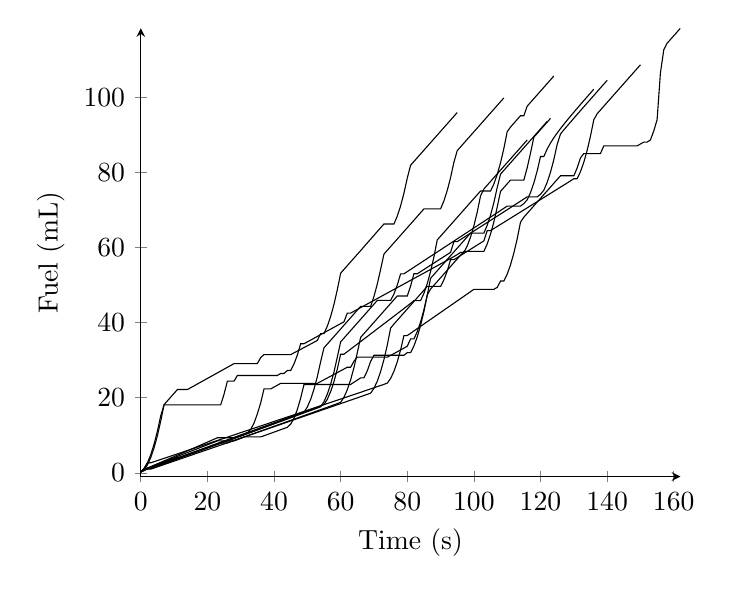
\begin{tikzpicture}
\begin{axis}[
legend style={anchor=west},
axis x line=bottom,
axis y line=left,
ymin=-1,
xlabel=Time (s),
ylabel=Fuel (mL),
]
\addplot[] coordinates {
(0, 0.239885513361)
(1, 0.766617621116)
(2, 1.08709758181)
(3, 1.40758497837)
(4, 1.72808020027)
(5, 2.04858366472)
(6, 2.36909581918)
(7, 2.68961714422)
(8, 3.01014815659)
(9, 3.33068941274)
(10, 3.6512415127)
(11, 3.97180510443)
(12, 4.29238088878)
(13, 4.61296962496)
(14, 4.93357213677)
(15, 5.25418931972)
(16, 5.57482214894)
(17, 5.89547168835)
(18, 6.21613910102)
(19, 6.53682566105)
(20, 6.85753276724)
(21, 7.17826195881)
(22, 7.49901493359)
(23, 7.81979356912)
(24, 8.14059994722)
(25, 8.46143638284)
(26, 8.78230545781)
(27, 9.10453591631)
(28, 9.4276709852)
(29, 9.75116298729)
(30, 10.0737554582)
(31, 10.3963723276)
(32, 10.7190161515)
(33, 11.04168986)
(34, 11.3643968287)
(35, 11.6871409684)
(36, 12.0099268366)
(37, 12.3327597795)
(38, 12.655646113)
(39, 12.978593358)
(40, 13.3016105483)
(41, 13.6247086404)
(42, 13.9479010682)
(43, 14.2712045075)
(44, 14.5946399521)
(45, 14.918234265)
(46, 15.2420224816)
(47, 15.5660513463)
(48, 15.8903849693)
(49, 16.2151143487)
(50, 16.5403744605)
(51, 16.8663776308)
(52, 17.1934867013)
(53, 17.522405092)
(54, 17.8548280695)
(55, 18.1973707627)
(56, 19.595563849)
(57, 21.6312611565)
(58, 24.3053215731)
(59, 27.6250572516)
(60, 31.6042336095)
(61, 31.6042336095)
(62, 32.2792361189)
(63, 32.9542416009)
(64, 33.6292505828)
(65, 34.3042637193)
(66, 34.9792818336)
(67, 35.6543059721)
(68, 36.3293374845)
(69, 37.0043781377)
(70, 37.6794302852)
(71, 38.3544971234)
(72, 39.029583091)
(73, 39.7046945116)
(74, 40.3798406682)
(75, 41.0557239752)
(76, 41.732784354)
(77, 42.4108338501)
(78, 43.0904833237)
(79, 43.7729239316)
(80, 44.4607689175)
(81, 45.1608350129)
(82, 45.8944650363)
(83, 45.8944650363)
(84, 45.8944650363)
(85, 47.8396063179)
(86, 50.422594991)
(87, 53.6498255499)
(88, 57.534145754)
(89, 62.0576642363)
(90, 63.0616540993)
(91, 64.0656439623)
(92, 65.0696338253)
(93, 66.0736236884)
(94, 67.0776135514)
(95, 68.0816034144)
(96, 69.0855932774)
(97, 70.0895831405)
(98, 71.0935730035)
(99, 72.0975628665)
(100, 73.1015527295)
(101, 74.1055425925)
(102, 75.1095324556)
(103, 75.1095324556)
(104, 75.1095324556)
(105, 75.1095324556)
(106, 76.978263322)
(107, 79.4845079301)
(108, 82.6338864636)
(109, 86.4384723714)
(110, 90.9167923671)
(111, 92.1580150926)
(112, 93.1620049556)
(113, 94.1659948186)
(114, 95.1699846817)
(115, 95.1699846817)
(116, 97.7152725592)
(117, 98.7192624222)
(118, 99.7232522853)
(119, 100.727242148)
(120, 101.731232011)
(121, 102.735221874)
(122, 103.739211737)
(123, 104.7432016)
(124, 105.747191463)
};
\addplot[] coordinates {
(0, 0.239885513361)
(1, 0.721796247693)
(2, 1.0358082283)
(3, 1.34982637617)
(4, 1.66385098473)
(5, 1.97788236635)
(6, 2.29192085391)
(7, 2.60596680255)
(8, 2.92002059156)
(9, 3.23408262644)
(10, 3.54815334123)
(11, 3.8622332011)
(12, 4.17632270518)
(13, 4.49042238972)
(14, 4.80453283163)
(15, 5.11865465244)
(16, 5.43278852269)
(17, 5.74693516691)
(18, 6.06109536916)
(19, 6.37526997933)
(20, 6.68945992023)
(21, 7.0036661956)
(22, 7.31788989928)
(23, 7.63213222558)
(24, 7.94639448118)
(25, 7.94639448118)
(26, 7.94639448118)
(27, 8.27747161143)
(28, 8.59219066325)
(29, 8.90742530016)
(30, 9.22370449251)
(31, 9.54064186901)
(32, 9.85737353126)
(33, 10.1737064241)
(34, 10.4900600247)
(35, 10.8064363194)
(36, 11.1228375603)
(37, 11.4392663111)
(38, 11.7557255038)
(39, 12.072218509)
(40, 12.3887492212)
(41, 12.7053221678)
(42, 13.0219426446)
(43, 13.3386168902)
(44, 13.6553523102)
(45, 13.9721577711)
(46, 14.2890439889)
(47, 14.6060240543)
(48, 14.9231141531)
(49, 15.2403345763)
(50, 15.5577111711)
(51, 15.8752774856)
(52, 16.1930780482)
(53, 16.5111735901)
(54, 16.8296497965)
(55, 17.1486329395)
(56, 17.4683202589)
(57, 17.7890462403)
(58, 18.11145389)
(59, 18.4370782708)
(60, 18.7718404678)
(61, 20.132860248)
(62, 22.131532813)
(63, 24.7683418673)
(64, 28.0502243804)
(65, 31.9905705868)
(66, 36.0839399334)
(67, 37.0879297965)
(68, 38.0919196595)
(69, 39.0959095225)
(70, 40.0998993855)
(71, 41.1038892486)
(72, 42.1078791116)
(73, 43.1118689746)
(74, 44.1158588376)
(75, 45.1198487006)
(76, 46.1238385637)
(77, 47.1278284267)
(78, 47.1278284267)
(79, 47.1278284267)
(80, 47.1278284267)
(81, 49.7619304093)
(82, 53.041062953)
(83, 53.041062953)
(84, 53.6124281296)
(85, 54.1837933355)
(86, 54.7551585738)
(87, 55.3265238478)
(88, 55.8978891615)
(89, 56.4692545192)
(90, 57.0406742607)
(91, 57.6120547424)
(92, 58.1834268074)
(93, 58.754798918)
(94, 61.6018599133)
(95, 61.6018599133)
(96, 62.1690141416)
(97, 62.7361859918)
(98, 63.3033783496)
(99, 63.8705947484)
(100, 64.4378395577)
(101, 65.0051182398)
(102, 65.5724377052)
(103, 66.1398068138)
(104, 66.7072370948)
(105, 67.2747438028)
(106, 67.8423475078)
(107, 68.4100765519)
(108, 68.9779709701)
(109, 69.5460889807)
(110, 70.1145181976)
(111, 70.6833960192)
(112, 71.2529490718)
(113, 71.8235756346)
(114, 72.3954060082)
(115, 72.9721206516)
(116, 73.555576238)
(117, 73.555576238)
(118, 73.555576238)
(119, 73.555576238)
(120, 74.2240216111)
(121, 75.3210347799)
(122, 77.398241346)
(123, 80.1140910005)
(124, 83.4763164865)
(125, 87.4991038124)
(126, 90.3186177379)
(127, 91.3829197557)
(128, 92.4304792154)
(129, 93.4660854342)
(130, 94.4930927181)
(131, 95.5138796674)
(132, 96.5301485974)
(133, 97.5431261577)
(134, 98.5537007135)
(135, 99.5625180369)
(136, 100.570048844)
(137, 101.576636944)
(138, 102.582533827)
(139, 103.587923657)
(140, 104.596899343)
};
\addplot[] coordinates {
(0, 0.239885513361)
(1, 0.841669203293)
(2, 1.17158097305)
(3, 1.50150231265)
(4, 1.83143379257)
(5, 2.16137602963)
(6, 2.49132969183)
(7, 2.82129550378)
(8, 3.15127425287)
(9, 3.48126679619)
(10, 3.81127406847)
(11, 4.14129709111)
(12, 4.14129709111)
(13, 4.47093324678)
(14, 4.80057872468)
(15, 5.130234237)
(16, 5.45990057065)
(17, 5.78957859733)
(18, 6.11926928537)
(19, 6.44897371352)
(20, 6.77869308723)
(21, 7.10842875797)
(22, 7.43818224613)
(23, 7.76795526841)
(24, 8.09903345715)
(25, 8.43193196978)
(26, 8.43193196978)
(27, 8.78943402268)
(28, 9.12186908749)
(29, 9.45431543139)
(30, 9.78677447663)
(31, 10.1192478976)
(32, 10.4517376797)
(33, 10.7842461966)
(34, 11.1167763109)
(35, 11.4493315094)
(36, 11.7819160864)
(37, 12.114535397)
(38, 12.4471962146)
(39, 12.7799072486)
(40, 13.1126799133)
(41, 13.4455295114)
(42, 13.7784771269)
(43, 14.1115528111)
(44, 14.4448012843)
(45, 14.7782930166)
(46, 15.1121483137)
(47, 15.4465990161)
(48, 15.7821949679)
(49, 16.1209905479)
(50, 17.5334240011)
(51, 19.5833105246)
(52, 22.2716527829)
(53, 25.6059067053)
(54, 29.5999814862)
(55, 33.3061568052)
(56, 34.3101466682)
(57, 35.3141365312)
(58, 36.3181263943)
(59, 37.3221162573)
(60, 38.3261061203)
(61, 39.3300959833)
(62, 40.3340858463)
(63, 41.3380757094)
(64, 42.3420655724)
(65, 43.3460554354)
(66, 44.3500452984)
(67, 44.3500452984)
(68, 44.3500452984)
(69, 44.3500452984)
(70, 46.9911366921)
(71, 50.2773696364)
(72, 54.2221775082)
(73, 58.282460115)
(74, 59.2864499781)
(75, 60.2904398411)
(76, 61.2944297041)
(77, 62.2984195671)
(78, 63.3024094302)
(79, 64.3063992932)
(80, 65.3103891562)
(81, 66.3143790192)
(82, 67.3183688823)
(83, 68.3223587453)
(84, 69.3263486083)
(85, 70.3303384713)
(86, 70.3303384713)
(87, 70.3303384713)
(88, 70.3303384713)
(89, 70.3303384713)
(90, 70.3303384713)
(91, 72.4648003665)
(92, 75.2383364436)
(93, 78.659259489)
(94, 82.7423355536)
(95, 85.8598887676)
(96, 86.8638786306)
(97, 87.8678684936)
(98, 88.8718583566)
(99, 89.8758482197)
(100, 90.8798380827)
(101, 91.8838279457)
(102, 92.8878178087)
(103, 93.8918076718)
(104, 94.8957975348)
(105, 95.8997873978)
(106, 96.9037772608)
(107, 97.9077671239)
(108, 98.9117569869)
(109, 99.9157468499)
};
\addplot[] coordinates {
(0, 0.239885513361)
(1, 1.13183007041)
(2, 2.66515136892)
(3, 2.66515136892)
(4, 2.96235257606)
(5, 3.25955820712)
(6, 3.55676843281)
(7, 3.85398343273)
(8, 4.15120339604)
(9, 4.44842852202)
(10, 4.74565902083)
(11, 5.04289511423)
(12, 5.34013703641)
(13, 5.63738503487)
(14, 5.93463937137)
(15, 6.23190032301)
(16, 6.52916818334)
(17, 6.82644326363)
(18, 7.12372589422)
(19, 7.42101642604)
(20, 7.71831523218)
(21, 8.01562270977)
(22, 8.31293928188)
(23, 8.61026539973)
(24, 8.90760154507)
(25, 9.20494823284)
(26, 9.50230601407)
(27, 9.79967547914)
(28, 10.0970572614)
(29, 10.3944520411)
(30, 10.6918605499)
(31, 10.9892835761)
(32, 11.2867219696)
(33, 11.584487037)
(34, 11.8827476291)
(35, 12.1813654198)
(36, 12.480364028)
(37, 12.7791215077)
(38, 13.0778021433)
(39, 13.3764940493)
(40, 13.675198016)
(41, 13.9739149096)
(42, 14.2726456827)
(43, 14.5713913849)
(44, 14.8701531758)
(45, 15.1689323401)
(46, 15.4677303049)
(47, 15.7665486608)
(48, 16.0653891859)
(49, 16.3642538755)
(50, 16.6631449759)
(51, 16.9620650271)
(52, 17.2610169129)
(53, 17.5600039227)
(54, 17.8590298276)
(55, 18.1580989739)
(56, 18.4572164013)
(57, 18.7563879913)
(58, 19.0556206571)
(59, 19.3549225898)
(60, 19.6543035811)
(61, 19.9537754542)
(62, 20.2533526483)
(63, 20.5530530291)
(64, 20.8528990394)
(65, 21.15291938)
(66, 21.4531515465)
(67, 21.7536458203)
(68, 22.0544718671)
(69, 22.3557303682)
(70, 22.6575753117)
(71, 22.9602619193)
(72, 23.2642685836)
(73, 23.5707050723)
(74, 23.8837013296)
(75, 25.1400136243)
(76, 27.0345137512)
(77, 29.5666297562)
(78, 32.7422429499)
(79, 36.5736879078)
(80, 36.5736879078)
(81, 37.1894854606)
(82, 37.8052847332)
(83, 38.4210859741)
(84, 39.0368894804)
(85, 39.6526956109)
(86, 40.2685048014)
(87, 40.8843175871)
(88, 41.5001346311)
(89, 42.1159567648)
(90, 42.7317850424)
(91, 43.3476208197)
(92, 43.963465866)
(93, 44.5793225301)
(94, 45.1951939904)
(95, 45.8110846423)
(96, 46.4270364848)
(97, 47.0439221787)
(98, 47.6612467951)
(99, 48.2792081915)
(100, 48.89813525)
(101, 48.89813525)
(102, 48.89813525)
(103, 48.89813525)
(104, 48.89813525)
(105, 48.89813525)
(106, 48.89813525)
(107, 49.4127215327)
(108, 51.1084813475)
(109, 51.1084813475)
(110, 52.9547626197)
(111, 55.4384772704)
(112, 58.5650180069)
(113, 62.3462308016)
(114, 66.8004148913)
(115, 68.1235435499)
(116, 69.1275334129)
(117, 70.131523276)
(118, 71.135513139)
(119, 72.139503002)
(120, 73.143492865)
(121, 74.1474827281)
(122, 75.1514725911)
(123, 76.1554624541)
(124, 77.1594523171)
(125, 78.1634421802)
(126, 79.1674320432)
(127, 79.1674320432)
(128, 79.1674320432)
(129, 79.1674320432)
(130, 79.1674320432)
(131, 81.2350104653)
(132, 83.9411645953)
(133, 85.0856655006)
(134, 85.0856655006)
(135, 85.0856655006)
(136, 85.0856655006)
(137, 85.0856655006)
(138, 85.0856655006)
(139, 87.1302386009)
(140, 87.1302386009)
(141, 87.1302386009)
(142, 87.1302386009)
(143, 87.1302386009)
(144, 87.1302386009)
(145, 87.1302386009)
(146, 87.1302386009)
(147, 87.1302386009)
(148, 87.1302386009)
(149, 87.1302386009)
(150, 87.6344866857)
(151, 88.1387810755)
(152, 88.1387810755)
(153, 88.7285525069)
(154, 91.1042606744)
(155, 94.1214294934)
(156, 106.573118119)
(157, 112.70473431)
(158, 114.476541069)
(159, 115.480530932)
(160, 116.484520795)
(161, 117.488510658)
(162, 118.492500521)
};
\addplot[] coordinates {
(0, 0.239885513361)
(1, 0.670769182584)
(2, 0.97634956868)
(3, 0.97634956868)
(4, 1.28173702068)
(5, 1.58712693446)
(6, 1.89251941507)
(7, 2.19791457363)
(8, 2.5033125278)
(9, 2.80871340223)
(10, 3.11411732915)
(11, 3.4195244489)
(12, 3.72493491058)
(13, 4.03034887276)
(14, 4.33576650425)
(15, 4.64118798492)
(16, 4.94661350664)
(17, 5.25204327429)
(18, 5.5574775069)
(19, 5.86291643891)
(20, 6.16836032151)
(21, 6.47380942422)
(22, 6.77926403658)
(23, 7.08472447004)
(24, 7.39019106012)
(25, 7.69566416876)
(26, 8.001144187)
(27, 8.30663153799)
(28, 8.61212668037)
(29, 8.9176301121)
(30, 9.22314237479)
(31, 9.52866405863)
(32, 9.83419580801)
(33, 10.1405566481)
(34, 10.4475696363)
(35, 10.7551515939)
(36, 11.0626101217)
(37, 11.3697363697)
(38, 11.6768674172)
(39, 11.9840036593)
(40, 12.2911455359)
(41, 12.5982935385)
(42, 12.9054482185)
(43, 13.2126101959)
(44, 13.5197801716)
(45, 13.8269589402)
(46, 14.1341474068)
(47, 14.4413466077)
(48, 14.7485577349)
(49, 15.0557821674)
(50, 15.3630215103)
(51, 15.6702776442)
(52, 15.9775527885)
(53, 16.2848495839)
(54, 16.5921712007)
(55, 16.8995214837)
(56, 17.206905149)
(57, 17.5143280581)
(58, 17.8217976068)
(59, 18.1293232937)
(60, 18.4369175789)
(61, 18.7445972328)
(62, 19.0523855609)
(63, 19.3603163109)
(64, 19.6684411138)
(65, 19.9768453387)
(66, 20.2856878897)
(67, 20.5953316392)
(68, 20.9070759547)
(69, 21.2222070277)
(70, 22.5016131427)
(71, 24.4190743231)
(72, 26.9742512933)
(73, 30.1732580424)
(74, 34.0286618246)
(75, 38.5594831588)
(76, 39.6365881465)
(77, 40.6405780095)
(78, 41.6445678725)
(79, 42.6485577356)
(80, 43.6525475986)
(81, 44.6565374616)
(82, 45.6605273246)
(83, 46.6645171877)
(84, 47.6685070507)
(85, 48.6724969137)
(86, 49.6764867767)
(87, 49.6764867767)
(88, 49.6764867767)
(89, 49.6764867767)
(90, 49.6764867767)
(91, 51.413532691)
(92, 53.7877354245)
(93, 56.8033810707)
(94, 56.8033810707)
(95, 57.3587054684)
(96, 57.914030616)
(97, 58.4693565872)
(98, 59.0246834657)
(99, 59.5800113466)
(100, 60.1353403387)
(101, 60.6907425922)
(102, 61.2460821515)
(103, 61.8014232753)
(104, 64.5476058339)
(105, 64.5476058339)
(106, 65.0990555305)
(107, 65.650508463)
(108, 66.2019651102)
(109, 66.7534260481)
(110, 67.3048919746)
(111, 67.8563637437)
(112, 68.4078424104)
(113, 68.9593292917)
(114, 69.5108260517)
(115, 70.0623348211)
(116, 70.6138583682)
(117, 71.1654003496)
(118, 71.716965687)
(119, 72.2685611476)
(120, 72.8201962676)
(121, 73.371884877)
(122, 73.9236477226)
(123, 74.4755172155)
(124, 75.0275465627)
(125, 75.5798287059)
(126, 76.1324848557)
(127, 76.6859794371)
(128, 77.2411791602)
(129, 77.8009731661)
(130, 78.3807087889)
(131, 78.3807087889)
(132, 80.2519865043)
(133, 82.760787585)
(134, 85.9127580223)
(135, 89.7199970722)
(136, 94.1021001543)
(137, 95.6943595191)
(138, 96.6983493821)
(139, 97.7023392451)
(140, 98.7063291081)
(141, 99.7103189712)
(142, 100.714308834)
(143, 101.718298697)
(144, 102.72228856)
(145, 103.726278423)
(146, 104.730268286)
(147, 105.734258149)
(148, 106.738248012)
(149, 107.742237875)
(150, 108.746227738)
};
\addplot[] coordinates {
(0, 0.239885513361)
(1, 0.777249275829)
(2, 1.09916109643)
(3, 1.09916109643)
(4, 1.42083073583)
(5, 1.74250449665)
(6, 2.06418260723)
(7, 2.38586531317)
(8, 2.70755287895)
(9, 3.02924558978)
(10, 3.35094375371)
(11, 3.67264770398)
(12, 3.99435780158)
(13, 4.31607443831)
(14, 4.63779804008)
(15, 4.95952907074)
(16, 5.28126803643)
(17, 5.60301549053)
(18, 5.92477203929)
(19, 6.24653834839)
(20, 6.56831515041)
(21, 6.89010325348)
(22, 7.21190355137)
(23, 7.53371703518)
(24, 7.85554480707)
(25, 8.17738809635)
(26, 8.49964170991)
(27, 8.82363175312)
(28, 9.14855358767)
(29, 9.47292146148)
(30, 9.7967562352)
(31, 10.1205993543)
(32, 10.4444517281)
(33, 10.7683144046)
(34, 11.092188598)
(35, 11.4160757233)
(36, 11.7399774405)
(37, 12.063895711)
(38, 12.3878328698)
(39, 12.7117917215)
(40, 13.0357756666)
(41, 13.3597888728)
(42, 13.6838365106)
(43, 14.0079250838)
(44, 14.3320629048)
(45, 14.656260798)
(46, 14.980533174)
(47, 15.3048997392)
(48, 15.6293883526)
(49, 15.9540401062)
(50, 16.2789191321)
(51, 16.6041337774)
(52, 16.9298904791)
(53, 17.2566728275)
(54, 17.586263063)
(55, 18.949459745)
(56, 20.9502999127)
(57, 23.5892892364)
(58, 26.873386651)
(59, 30.8160043567)
(60, 34.8925074388)
(61, 35.8964973018)
(62, 36.9004871648)
(63, 37.9044770279)
(64, 38.9084668909)
(65, 39.9124567539)
(66, 40.9164466169)
(67, 41.92043648)
(68, 42.924426343)
(69, 43.928416206)
(70, 44.932406069)
(71, 45.936395932)
(72, 45.936395932)
(73, 45.936395932)
(74, 45.936395932)
(75, 45.936395932)
(76, 47.6641271901)
(77, 50.029000469)
(78, 53.0352075251)
(79, 53.0352075251)
(80, 53.6168144616)
(81, 54.1984223644)
(82, 54.780031339)
(83, 55.3616415068)
(84, 55.9432530078)
(85, 56.5249400445)
(86, 57.1065719349)
(87, 57.6881971597)
(88, 58.2698245781)
(89, 58.8516760992)
(90, 59.4333349549)
(91, 60.014997971)
(92, 60.596665832)
(93, 61.1783393771)
(94, 61.7600196447)
(95, 62.3417079339)
(96, 62.9234058898)
(97, 63.5051156238)
(98, 64.0868398857)
(99, 64.6685823181)
(100, 65.2503478381)
(101, 65.8321432289)
(102, 66.4139780839)
(103, 66.9958663721)
(104, 67.5778291433)
(105, 68.1598994518)
(106, 68.7421318834)
(107, 69.3246224531)
(108, 69.9075544174)
(109, 70.4912375548)
(110, 71.0767812554)
(111, 71.0767812554)
(112, 71.0767812554)
(113, 71.0767812554)
(114, 71.0767812554)
(115, 71.7536799432)
(116, 72.7557925884)
(117, 74.6780304866)
(118, 77.2380060142)
(119, 80.4418815665)
(120, 84.3022728038)
(121, 84.3022728038)
(122, 86.2992025034)
(123, 87.9028200714)
(124, 89.2947124505)
(125, 90.5602805216)
(126, 91.7455207615)
(127, 92.8774548978)
(128, 93.9729446596)
(129, 95.0429816874)
(130, 96.0949662386)
(131, 97.1340020973)
(132, 98.1636732279)
(133, 99.1865305011)
(134, 100.20440785)
(135, 101.221816107)
(136, 102.260816814)
};
\addplot[] coordinates {
(0, 0.239885513361)
(1, 0.573875905005)
(2, 1.15496767622)
(3, 1.55393223668)
(4, 2.01479615362)
(5, 2.39798838878)
(6, 2.78119837679)
(7, 3.1644281472)
(8, 3.54768005017)
(9, 3.93095682223)
(10, 4.31426166895)
(11, 4.69759836973)
(12, 5.08097141201)
(13, 5.46438616503)
(14, 5.84784910726)
(15, 6.23136812838)
(16, 6.61651710011)
(17, 7.01086030938)
(18, 7.40013707314)
(19, 7.78712181789)
(20, 8.17414954092)
(21, 8.5612307338)
(22, 8.94837960508)
(23, 9.33561589681)
(24, 9.33561589681)
(25, 9.33561589681)
(26, 9.33561589681)
(27, 9.33561589681)
(28, 9.33561589681)
(29, 9.66873214584)
(30, 10.002470679)
(31, 10.3372177663)
(32, 10.6745889968)
(33, 11.5401970537)
(34, 13.2600860483)
(35, 15.7080374648)
(36, 18.6336858649)
(37, 22.3512890668)
(38, 22.3512890668)
(39, 22.3512890668)
(40, 22.8459874148)
(41, 23.3406883628)
(42, 23.8353921333)
(43, 23.8353921333)
(44, 23.8353921333)
(45, 23.8353921333)
(46, 23.8353921333)
(47, 23.8353921333)
(48, 23.8353921333)
(49, 23.8353921333)
(50, 23.8353921333)
(51, 23.8353921333)
(52, 23.8353921333)
(53, 23.8353921333)
(54, 24.3133636338)
(55, 24.7913510127)
(56, 25.2693516809)
(57, 25.7473652079)
(58, 26.2253923298)
(59, 26.7034345163)
(60, 27.1814938137)
(61, 27.6595728317)
(62, 28.1376748193)
(63, 28.1376748193)
(64, 29.7273615985)
(65, 30.816180488)
(66, 30.816180488)
(67, 30.816180488)
(68, 30.816180488)
(69, 30.816180488)
(70, 30.816180488)
(71, 30.816180488)
(72, 30.816180488)
(73, 30.816180488)
(74, 30.816180488)
(75, 31.2951668338)
(76, 31.7748334345)
(77, 32.2555191994)
(78, 32.7378374968)
(79, 33.224828662)
(80, 33.7285893298)
(81, 35.675716497)
(82, 35.675716497)
(83, 37.620338255)
(84, 40.2028048221)
(85, 43.429505428)
(86, 47.3132825672)
(87, 51.8411049818)
(88, 52.8450948448)
(89, 53.8490847078)
(90, 54.8530745708)
(91, 55.8570644339)
(92, 56.8610542969)
(93, 57.8650441599)
(94, 58.8690340229)
(95, 59.873023886)
(96, 60.877013749)
(97, 61.881003612)
(98, 62.884993475)
(99, 63.888983338)
(100, 63.888983338)
(101, 63.888983338)
(102, 63.888983338)
(103, 63.888983338)
(104, 65.9582563257)
(105, 68.6661167734)
(106, 72.0202170416)
(107, 76.0346627557)
(108, 79.6003740644)
(109, 80.6043639275)
(110, 81.6083537905)
(111, 82.6123436535)
(112, 83.6163335165)
(113, 84.6203233796)
(114, 85.6243132426)
(115, 86.6283031056)
(116, 87.6322929686)
(117, 88.6362828316)
(118, 89.6402726947)
(119, 90.6442625577)
(120, 91.6482524207)
(121, 92.6522422837)
(122, 93.6562321468)
};
\addplot[] coordinates {
(0, 0.239885513361)
(1, 0.954978135027)
(2, 1.29683412691)
(3, 1.63870293383)
(4, 1.98058544256)
(5, 2.32248262373)
(6, 2.66439554202)
(7, 3.00632536789)
(8, 3.348273391)
(9, 3.6902410359)
(10, 4.03222988013)
(11, 4.37424167545)
(12, 4.71627837255)
(13, 5.05834215031)
(14, 5.40043545022)
(15, 5.74256101736)
(16, 6.08472194933)
(17, 6.42692175493)
(18, 6.76916442512)
(19, 7.11145451924)
(20, 7.45379727057)
(21, 7.79717646909)
(22, 8.14314571515)
(23, 8.48944596301)
(24, 8.48944596301)
(25, 8.48944596301)
(26, 8.48944596301)
(27, 8.48944596301)
(28, 8.48944596301)
(29, 8.84547992202)
(30, 9.20152092991)
(31, 9.55759703252)
(32, 9.55759703252)
(33, 9.55759703252)
(34, 9.55759703252)
(35, 9.55759703252)
(36, 9.55759703252)
(37, 9.87755737656)
(38, 10.197696477)
(39, 10.5179981205)
(40, 10.8385062997)
(41, 11.1593104723)
(42, 11.4805812723)
(43, 11.802706969)
(44, 12.1270503677)
(45, 12.9719338416)
(46, 14.5244781328)
(47, 16.8836483577)
(48, 19.8840863198)
(49, 23.5363793679)
(50, 23.5363793679)
(51, 23.5363793679)
(52, 23.5363793679)
(53, 23.5363793679)
(54, 23.5363793679)
(55, 23.5363793679)
(56, 23.5363793679)
(57, 23.5363793679)
(58, 23.5363793679)
(59, 23.5363793679)
(60, 23.5363793679)
(61, 23.5363793679)
(62, 23.5363793679)
(63, 23.5363793679)
(64, 24.1262856254)
(65, 24.7162821077)
(66, 25.3063710179)
(67, 25.3063710179)
(68, 27.1744772553)
(69, 29.6800948898)
(70, 31.3282356667)
(71, 31.3282356667)
(72, 31.3282356667)
(73, 31.3282356667)
(74, 31.3282356667)
(75, 31.3282356667)
(76, 31.3282356667)
(77, 31.3282356667)
(78, 31.3282356667)
(79, 31.3282356667)
(80, 32.0208283985)
(81, 32.0208283985)
(82, 33.8059242619)
(83, 36.2282752043)
(84, 39.2926540315)
(85, 43.0102868141)
(86, 47.3988528877)
(87, 48.965469509)
(88, 49.969459372)
(89, 50.9734492351)
(90, 51.9774390981)
(91, 52.9814289611)
(92, 53.9854188241)
(93, 54.9894086872)
(94, 55.9933985502)
(95, 56.9973884132)
(96, 58.0013782762)
(97, 59.0053681393)
(98, 59.0053681393)
(99, 59.0053681393)
(100, 59.0053681393)
(101, 59.0053681393)
(102, 59.0053681393)
(103, 59.0053681393)
(104, 60.9893320848)
(105, 63.6113485427)
(106, 66.87820543)
(107, 70.8031439289)
(108, 75.0120894822)
(109, 76.0160793452)
(110, 77.0200692082)
(111, 78.0240590712)
(112, 78.0240590712)
(113, 78.0240590712)
(114, 78.0240590712)
(115, 78.0240590712)
(116, 81.2879215458)
(117, 85.2097898779)
(118, 89.4420101887)
(119, 90.4460000517)
(120, 91.4499899147)
(121, 92.4539797777)
(122, 93.4579696408)
(123, 94.4619595038)
};
\addplot[] coordinates {
(0, 0.239885513361)
(1, 1.13183007041)
(2, 2.66515136892)
(3, 4.83562037156)
(4, 7.64546130585)
(5, 11.1033516642)
(6, 15.2244222039)
(7, 18.1101790691)
(8, 18.1101790691)
(9, 18.1101790691)
(10, 18.1101790691)
(11, 18.1101790691)
(12, 18.1101790691)
(13, 18.1101790691)
(14, 18.1101790691)
(15, 18.1101790691)
(16, 18.1101790691)
(17, 18.1101790691)
(18, 18.1101790691)
(19, 18.1101790691)
(20, 18.1101790691)
(21, 18.1101790691)
(22, 18.1101790691)
(23, 18.1101790691)
(24, 18.1101790691)
(25, 20.9438611173)
(26, 24.4260385476)
(27, 24.4260385476)
(28, 24.4260385476)
(29, 25.9416404882)
(30, 25.9416404882)
(31, 25.9416404882)
(32, 25.9416404882)
(33, 25.9416404882)
(34, 25.9416404882)
(35, 25.9416404882)
(36, 25.9416404882)
(37, 25.9416404882)
(38, 25.9416404882)
(39, 25.9416404882)
(40, 25.9416404882)
(41, 25.9416404882)
(42, 26.4711136378)
(43, 26.4711136378)
(44, 27.2663384728)
(45, 27.2663384728)
(46, 29.0032521913)
(47, 31.3773225091)
(48, 34.3928341813)
(49, 34.3928341813)
(50, 34.8805264291)
(51, 35.3682186903)
(52, 35.8559109657)
(53, 36.3436032564)
(54, 36.8312955635)
(55, 37.3189878884)
(56, 37.8066802324)
(57, 38.2943725971)
(58, 38.7821008062)
(59, 39.2697981035)
(60, 39.757495418)
(61, 40.2451927512)
(62, 42.5669854804)
(63, 42.5669854804)
(64, 43.0516716423)
(65, 43.536363882)
(66, 44.0210628391)
(67, 44.5057692447)
(68, 44.9904839389)
(69, 45.4752078906)
(70, 45.9599422238)
(71, 46.4446882491)
(72, 46.9294475033)
(73, 47.4142218002)
(74, 47.8990132947)
(75, 48.383824566)
(76, 48.8686587251)
(77, 49.3535195577)
(78, 49.8384117137)
(79, 50.3233409645)
(80, 50.8083145561)
(81, 51.2933417019)
(82, 51.7784342852)
(83, 52.2636078789)
(84, 52.7488832629)
(85, 53.2342887427)
(86, 53.7198638001)
(87, 54.2056650504)
(88, 54.6917763714)
(89, 55.1783269949)
(90, 55.665183629)
(91, 56.1537812453)
(92, 56.643665958)
(93, 57.1365931458)
(94, 57.6358794235)
(95, 58.1519191625)
(96, 58.7421665511)
(97, 58.7421665511)
(98, 60.4634523491)
(99, 62.8218707357)
(100, 65.8215481916)
(101, 69.4730644624)
(102, 73.7934525583)
(103, 75.6457683677)
(104, 76.6497582307)
(105, 77.6537480938)
(106, 78.6577379568)
(107, 79.6617278198)
(108, 80.6657176828)
(109, 81.6697075459)
(110, 82.6736974089)
(111, 83.6776872719)
(112, 84.6816771349)
(113, 85.685666998)
(114, 86.689656861)
(115, 87.693646724)
(116, 88.697636587)
};
\addplot[] coordinates {
(0, 0.239885513361)
(1, 0.770600333171)
(2, 2.09972707916)
(3, 4.06665137892)
(4, 6.6715352084)
(5, 9.92099380841)
(6, 13.8280956846)
(7, 18.1734030458)
(8, 19.1773929088)
(9, 20.1813827718)
(10, 21.1853726348)
(11, 22.1893624979)
(12, 22.1893624979)
(13, 22.1893624979)
(14, 22.1893624979)
(15, 22.6826677054)
(16, 23.1759759944)
(17, 23.6692876433)
(18, 24.162602965)
(19, 24.6559223118)
(20, 25.1492460819)
(21, 25.6425747271)
(22, 26.1359087623)
(23, 26.6292487761)
(24, 27.122595445)
(25, 27.6159495496)
(26, 28.109311996)
(27, 28.6026838407)
(28, 29.0960663236)
(29, 29.0960663236)
(30, 29.0960663236)
(31, 29.0960663236)
(32, 29.0960663236)
(33, 29.0960663236)
(34, 29.0960663236)
(35, 29.0960663236)
(36, 30.7098180123)
(37, 31.5033042858)
(38, 31.5033042858)
(39, 31.5033042858)
(40, 31.5033042858)
(41, 31.5033042858)
(42, 31.5033042858)
(43, 31.5033042858)
(44, 31.5033042858)
(45, 31.5033042858)
(46, 31.9708846323)
(47, 32.4388424862)
(48, 32.9072118679)
(49, 33.3761605978)
(50, 33.8458036103)
(51, 34.3175048259)
(52, 34.7936775789)
(53, 35.2860259332)
(54, 37.0946259776)
(55, 37.0946259776)
(56, 39.053561759)
(57, 41.6504150686)
(58, 44.8917201928)
(59, 48.7904646826)
(60, 53.2006189129)
(61, 54.2046087759)
(62, 55.2085986389)
(63, 56.2125885019)
(64, 57.216578365)
(65, 58.220568228)
(66, 59.2183237393)
(67, 60.2385767083)
(68, 61.2544570662)
(69, 62.2671511642)
(70, 63.277518558)
(71, 64.3043019317)
(72, 65.3082917948)
(73, 66.3122816578)
(74, 66.3122816578)
(75, 66.3122816578)
(76, 66.3122816578)
(77, 68.4006221927)
(78, 71.1276855705)
(79, 74.5013173405)
(80, 78.5358163165)
(81, 81.9666063863)
(82, 82.9705962493)
(83, 83.9745861123)
(84, 84.9785759753)
(85, 85.9825658383)
(86, 86.9865557014)
(87, 87.9905455644)
(88, 88.9945354274)
(89, 89.9985252904)
(90, 91.0025151535)
(91, 92.0065050165)
(92, 93.0104948795)
(93, 94.0144847425)
(94, 95.0184746056)
(95, 96.0224644686)
};

\end{axis}
\end{tikzpicture}
\label{tik:fuel:100:51}
\caption{100 percent diving with GSC on route $51$}
\end{figure}


\begin{comment}
\begin{figure}
\begin{tikzpicture}[scale=1.3]
\begin{axis}[xlabel=Routes,xticklabel=\empty,ylabel=Fuel consumption,bar width=1pt,]
\addplot[ybar, blue] table[x=Route,y=Fuel] {TestResults/0/avg.dat};
\addplot[ybar, red] table[x=Route,y=Fuel] {TestResults/100/avg.dat};
\draw[thick, red] (axis cs:0,138) -- (axis cs:109,138);
\draw[thick, blue] (axis cs:0,162) -- (axis cs:109,162);
\end{axis}
\end{tikzpicture}
\caption{Average fuel consumption with (red) and without \tech (blue)}\label{tik:fuel:avg}
\end{figure}
\end{comment}


\subsection{Distance}
Figure~\ref{fig:TestResults:distance100} shows the distance ?? vehicles drive on route 54 as a function of time when their driving behaviour is solely controled by SUMO. 
The vehicle is stationary whenever the curve flatens.
From the figure we clearly see that the vehicles on this route has to stop four times, at 250 meter, at 550 meters, at 750 meters and again at 1100 metets.

When we control the speed of the vehicles using \tech, we see a different result showed in Figure~\ref{fig:TestResults:distance100}.
The curves in this figure are much more smooth, and fewer vehicles has to stop completely at a cross section.
Some vehicles have to stop due to blocking vehicles or cross traffic, which we do not take into account.

We can therefore see that using \tech results in less full stops.


\begin{figure}[htb]
\includegraphics[width=0.5\textwidth]{images/tp0/distance100.png}
\caption{Distance graph}
\label{fig:TestResults:distance100}
\end{figure}

\subsection{Speed}
Figure~\ref{fig:TestResults:speed0} shows the speed at which SUMO controlled vehicles on route 54 drive as a function over time.
The graph clearly shows that the vehicles quicly accelerates up to the maximal speed, then quickly decelerates to a full stop and then quickly accelerates again.
By using \tech we see a very different outline (See Figure~\ref{fig:TestResults:speed100}).
Few vehicles decelerates to $0 m/s$, and many stay above $5 m/s$ ($18 km/h$ or $11$ miles per hour ($mph$)).
We do, however, still see a large fluctuation.
\begin{figure}[htb]
\includegraphics[width=0.5\textwidth]{images/tp0/speed100.png}
\caption{Speed graph}
\label{fig:TestResults:speed100}
\end{figure}



\subsection{Time}
It is interesting to investigate wether driving after \tech results in longer travel time than without.
It takes on average 114 seconds to drive a route in our test without \tech, and when all vehicles drive with \tech it takes 111 seconds. 
We therefore do not see any significant differens in thees results.


